% Plant Physiology Supplemental Data (built by make_plantphys.py)
\documentclass[11pt]{article}
\usepackage[margin=2cm]{geometry}
\usepackage{graphicx}
\usepackage{caption}
\usepackage[authoryear,round]{natbib}
\usepackage{amsmath,amssymb}
\usepackage[hidelinks]{hyperref}
\captionsetup{labelformat=empty,font=small}
\begin{document}
\begin{center}
{\Large\textbf{Supplemental Data}}\\[6pt]
The aspartate-to-homoserine pathway recurs across maize grain amino acids, soil nitrogen, and yield selection\\[4pt]
Tandukar, Fitzsimmons, Flint-Garcia, Angelovici, and Rell\'an-\'Alvarez
\end{center}

\section*{Supplemental Figures}
\begin{figure}[p]
\centering
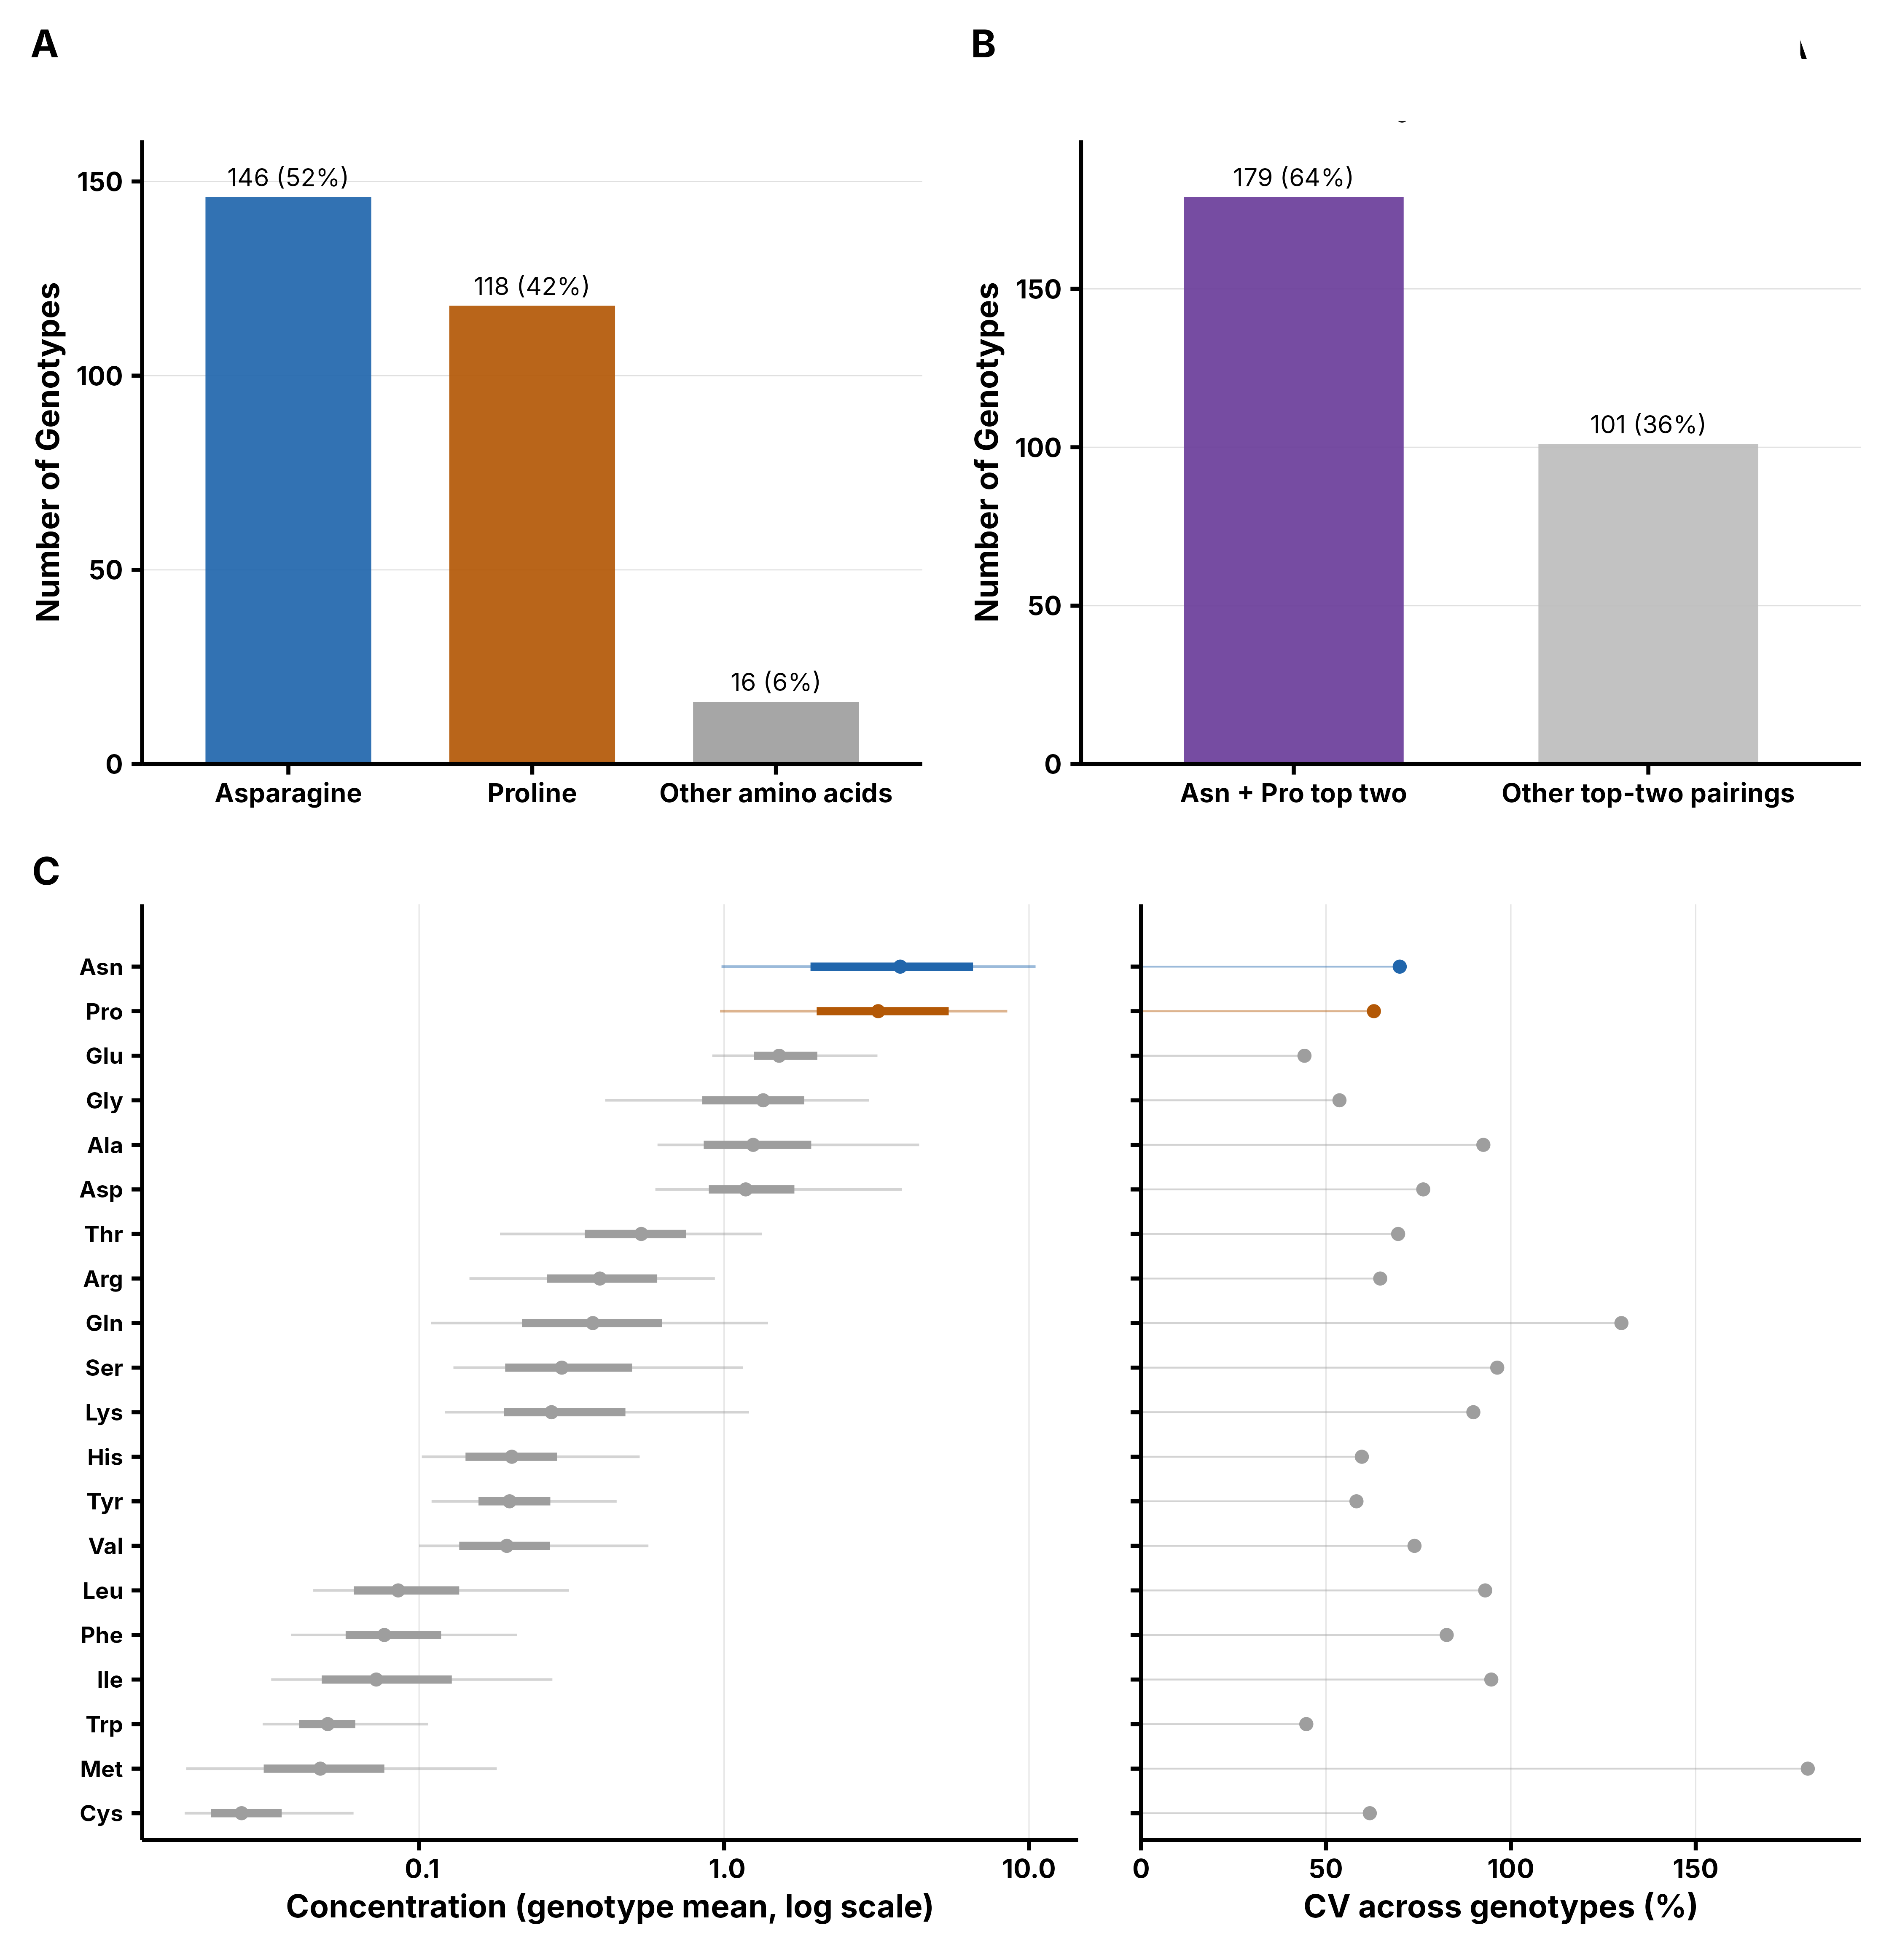
\includegraphics[width=0.95\textwidth]{../supp_figs/SuppFig1_FAA_composition.png}
\caption*{\textbf{Supplemental Figure S1.} \textbf{Free amino acid composition of the Goodman--Buckler panel.}
    \textbf{(A)}, Number of genotypes in which each free amino acid ranked most abundant,
    based on genotype means across four replicates ($n = 280$ genotypes).
    \textbf{(B)}, Number of genotypes in which Asn and Pro together occupied the
    top two ranks, in either order.
    \textbf{(C)}, Abundance and variability of each free amino acid. Left, concentration per
    genotype mean on a log scale: point, median across genotypes; thick bar, interquartile
    range; thin bar, 5th--95th percentile; amino acids ordered by median. Right,
    coefficient of variation across genotypes for the same ordering. Asn is shown in blue and Pro in orange throughout.}
\end{figure}
\clearpage

\begin{figure}[p]
\centering
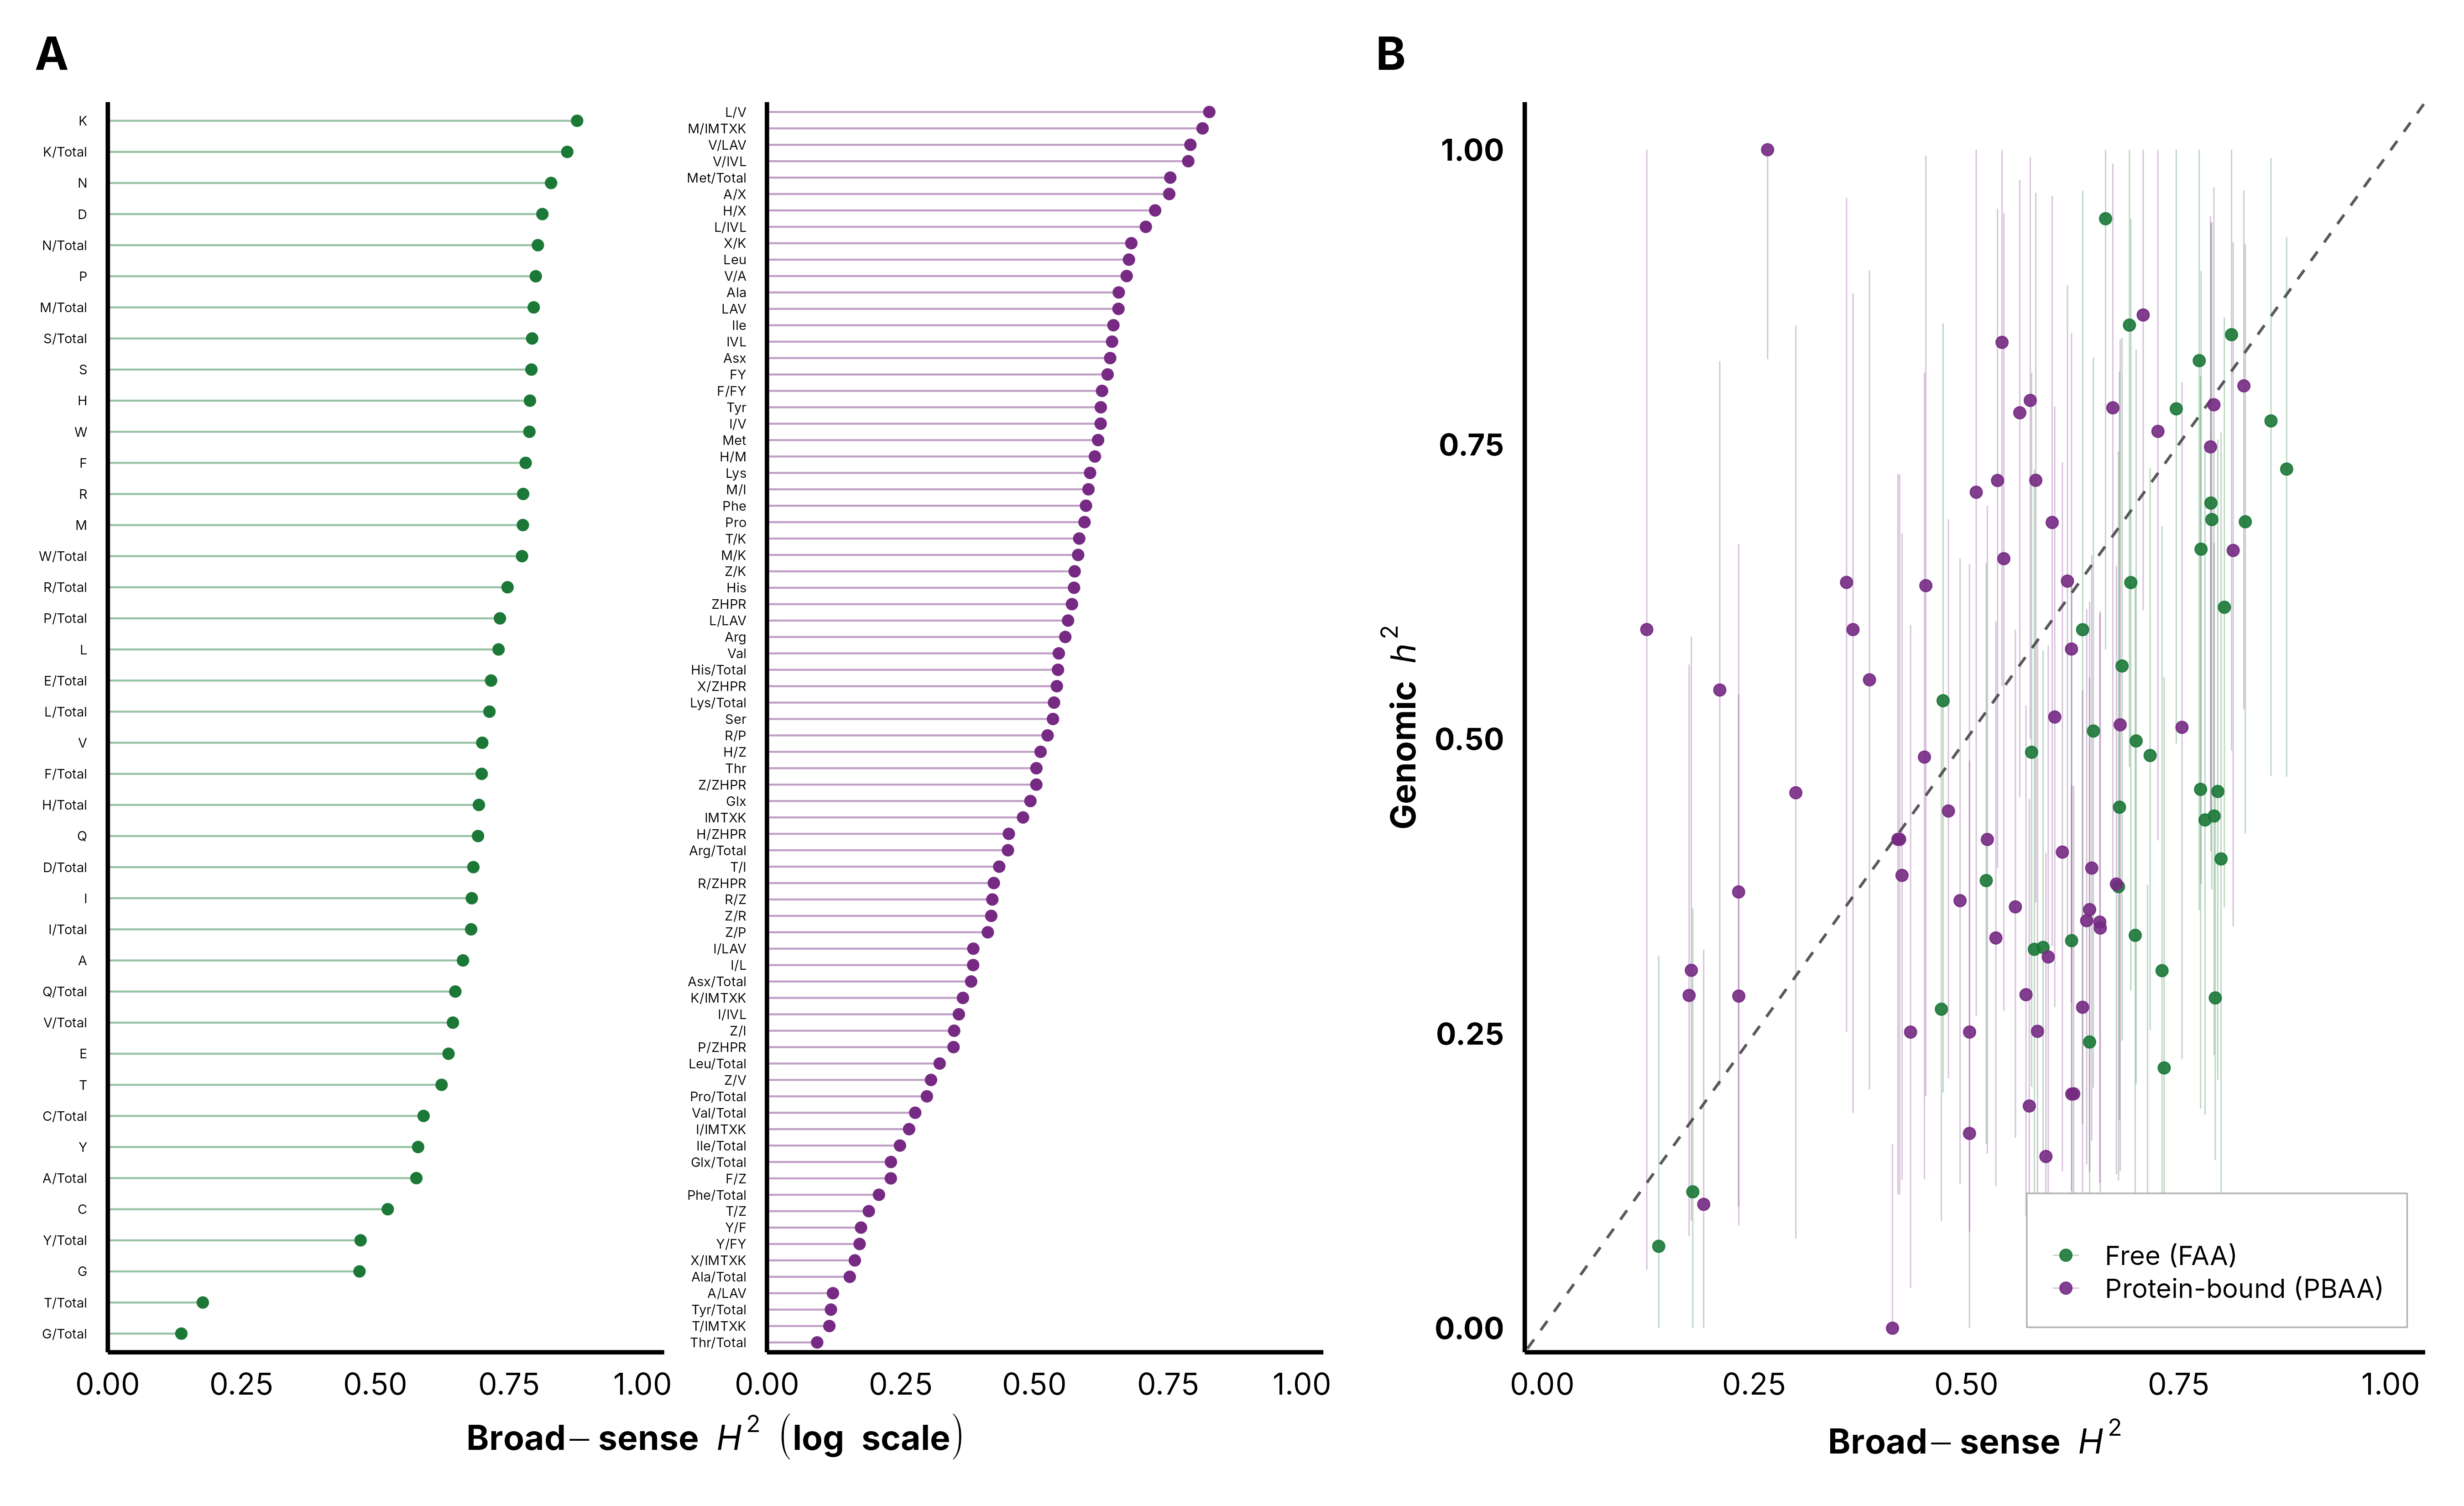
\includegraphics[width=\textwidth]{../supp_figs/SuppFig2_heritability.png}
\caption*{\textbf{Supplemental Figure S2.} \textbf{Heritability of grain amino acid phenotypes in the Goodman--Buckler panel.}
    \textbf{(A)}, Broad-sense heritability $H^2$ on a line-mean basis shown for 40 free and 76 protein-bound amino acid traits.
    \textbf{B}, Genomic heritability $h^2$ from a VanRaden genomic relationship matrix plotted against $H^2$, with error bars giving the 95\% profile-likelihood interval on $h^2$ and the dashed line showing $y = x$. Fifteen of
    116 traits returned a non-zero $h^2$ from a permuted phenotype and are excluded from
    panel \textbf{B}; their $H^2$ is unaffected and is retained in panel \textbf{A}.}
\end{figure}
\clearpage

\begin{figure}[p]
\centering
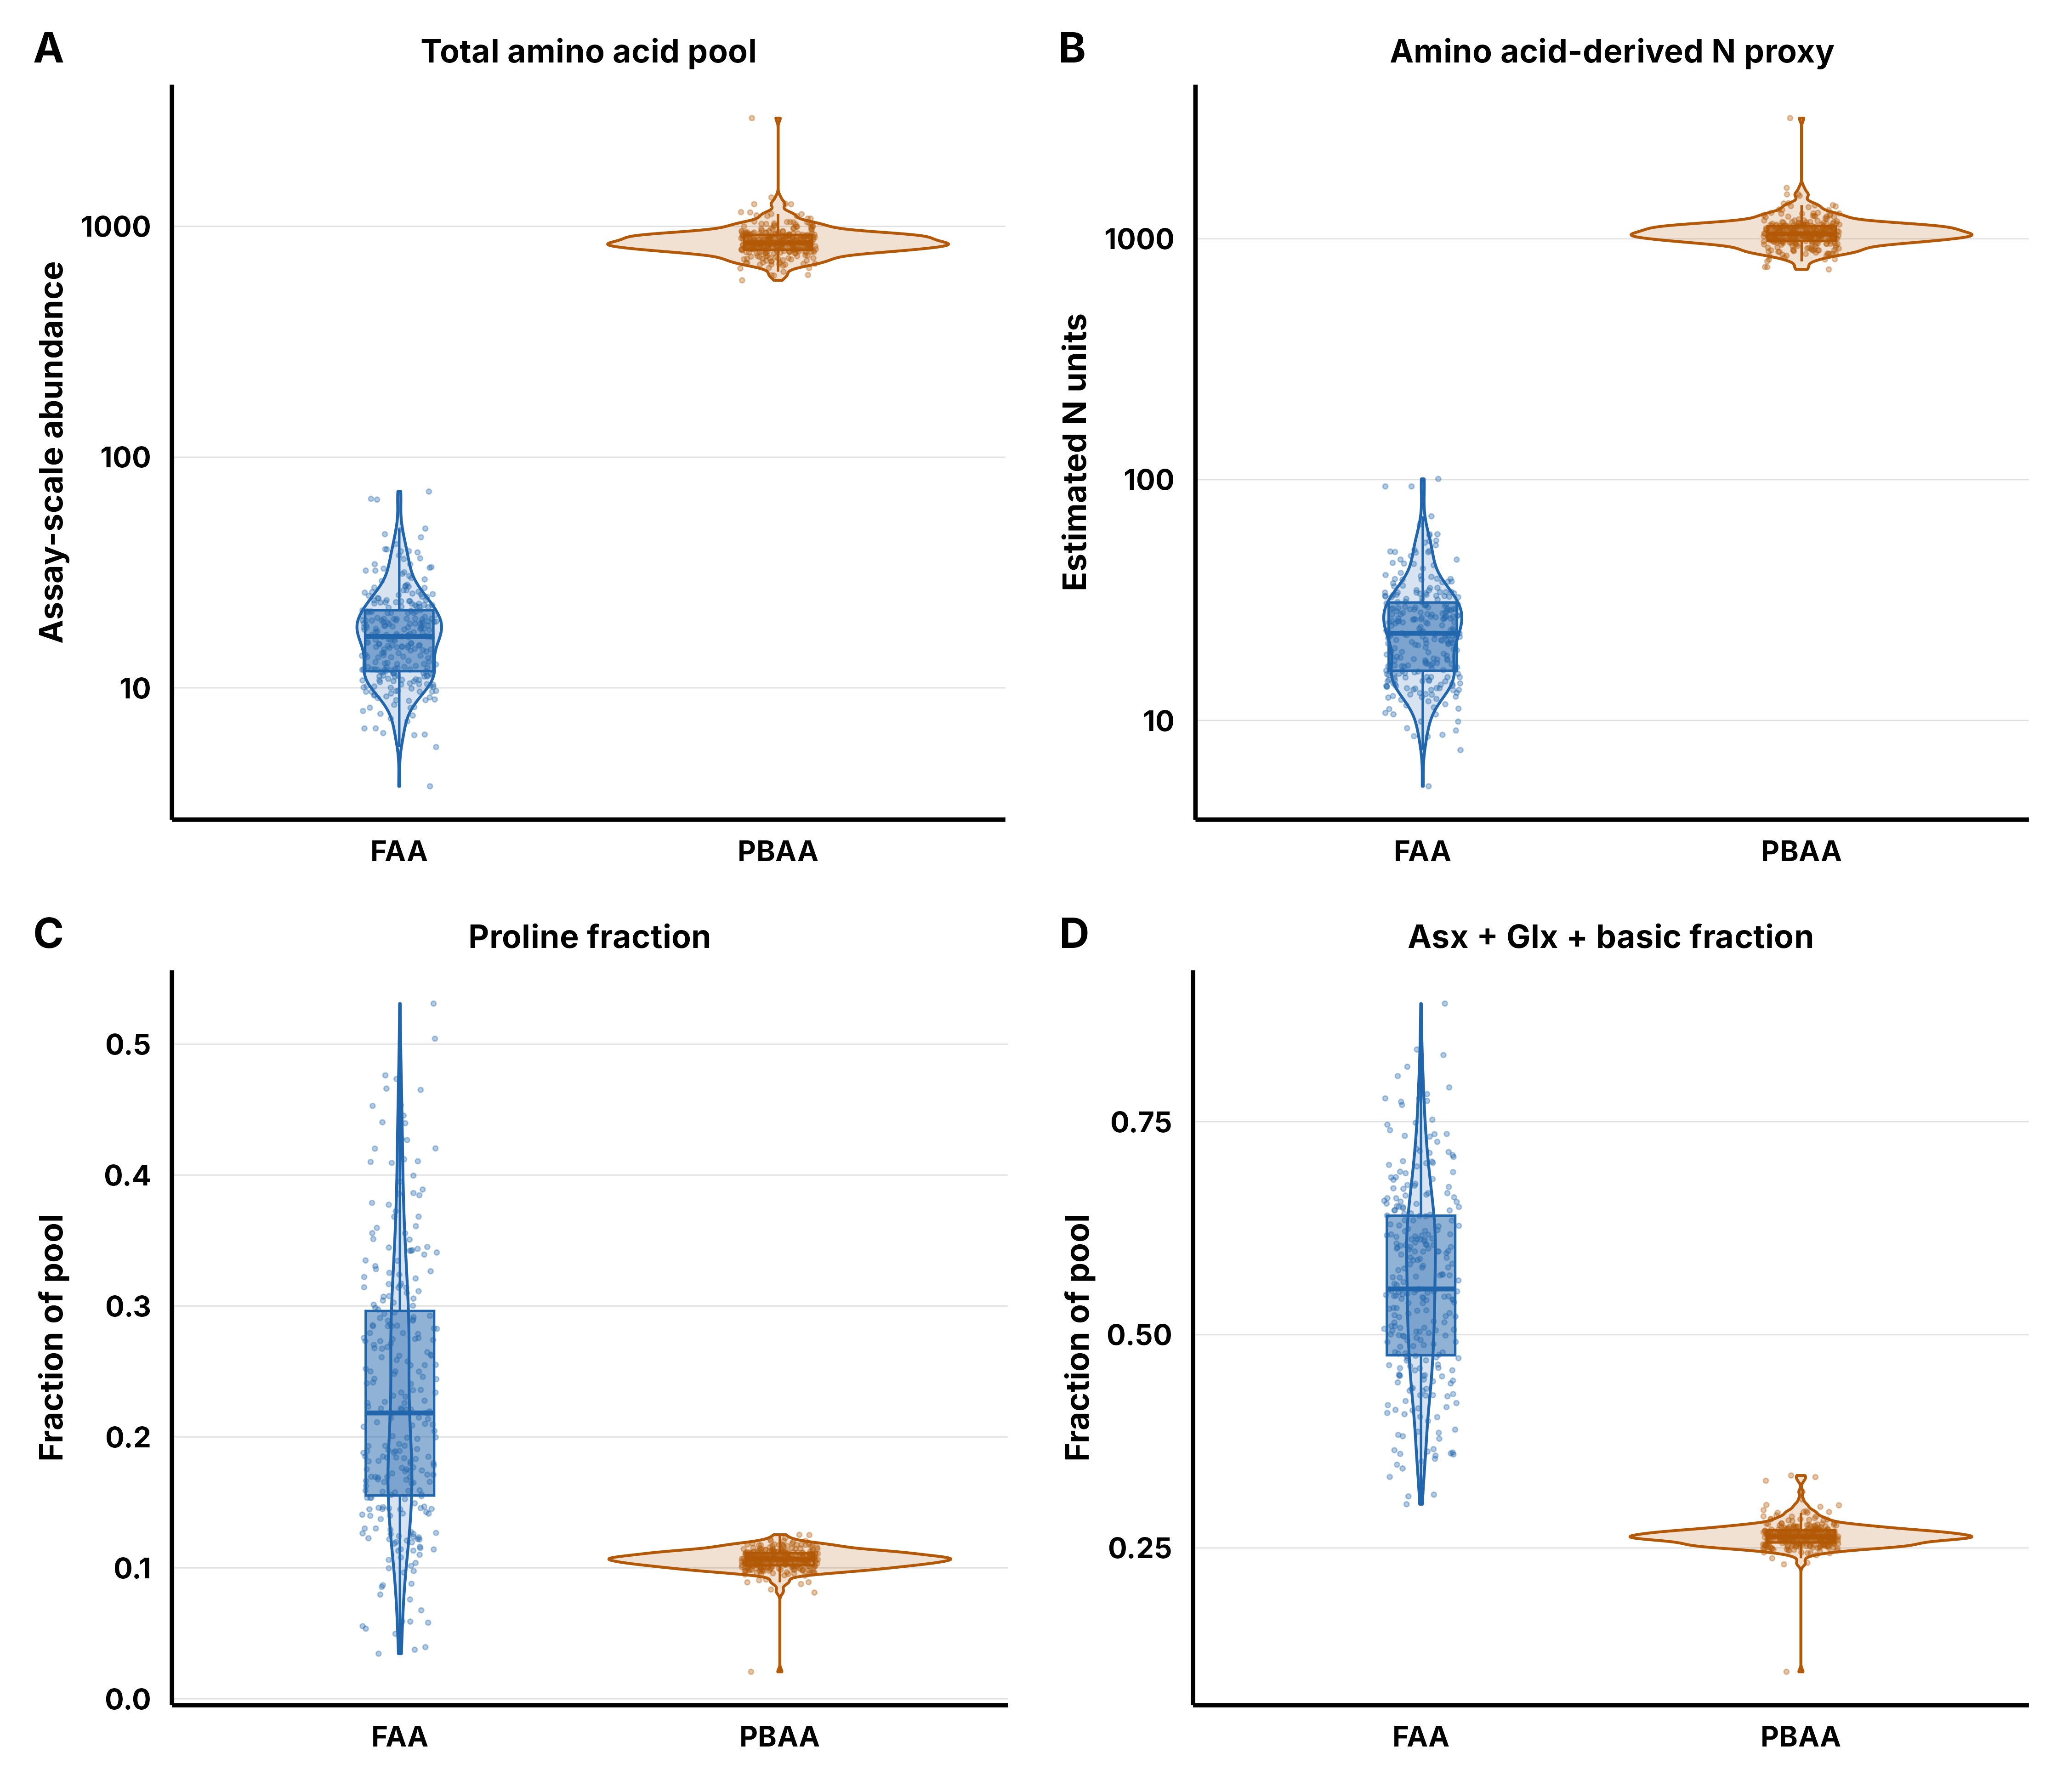
\includegraphics[width=\textwidth]{../supp_figs/SuppFig3_FAA_vs_PBAA_pools.png}
\caption*{\textbf{Supplemental Figure S3.} \textbf{Free (FAA) and protein-bound (PBAA) amino acid pools across matched Goodman--Buckler lines ($n = 279$)}. \textbf{(A)}, Total amino acid pool. \textbf{(B)}, Amino acid-derived N proxy, with each amino acid weighted by its number of N atoms (Asx and Glx, unresolved after acid
    hydrolysis, at 1.5 N). \textbf{(C)}, Proline fraction. \textbf{(D)}, Asx + Glx + basic
    (Arg, Lys, His) fraction. Fractions use matched denominators: free Asp + Asn and Glu + Gln
    are combined, and glycine, tryptophan and cysteine are excluded from the free-pool total. Violins show the distribution across lines and boxes the median and interquartile range.}
\end{figure}
\clearpage

\begin{figure}[p]
\centering
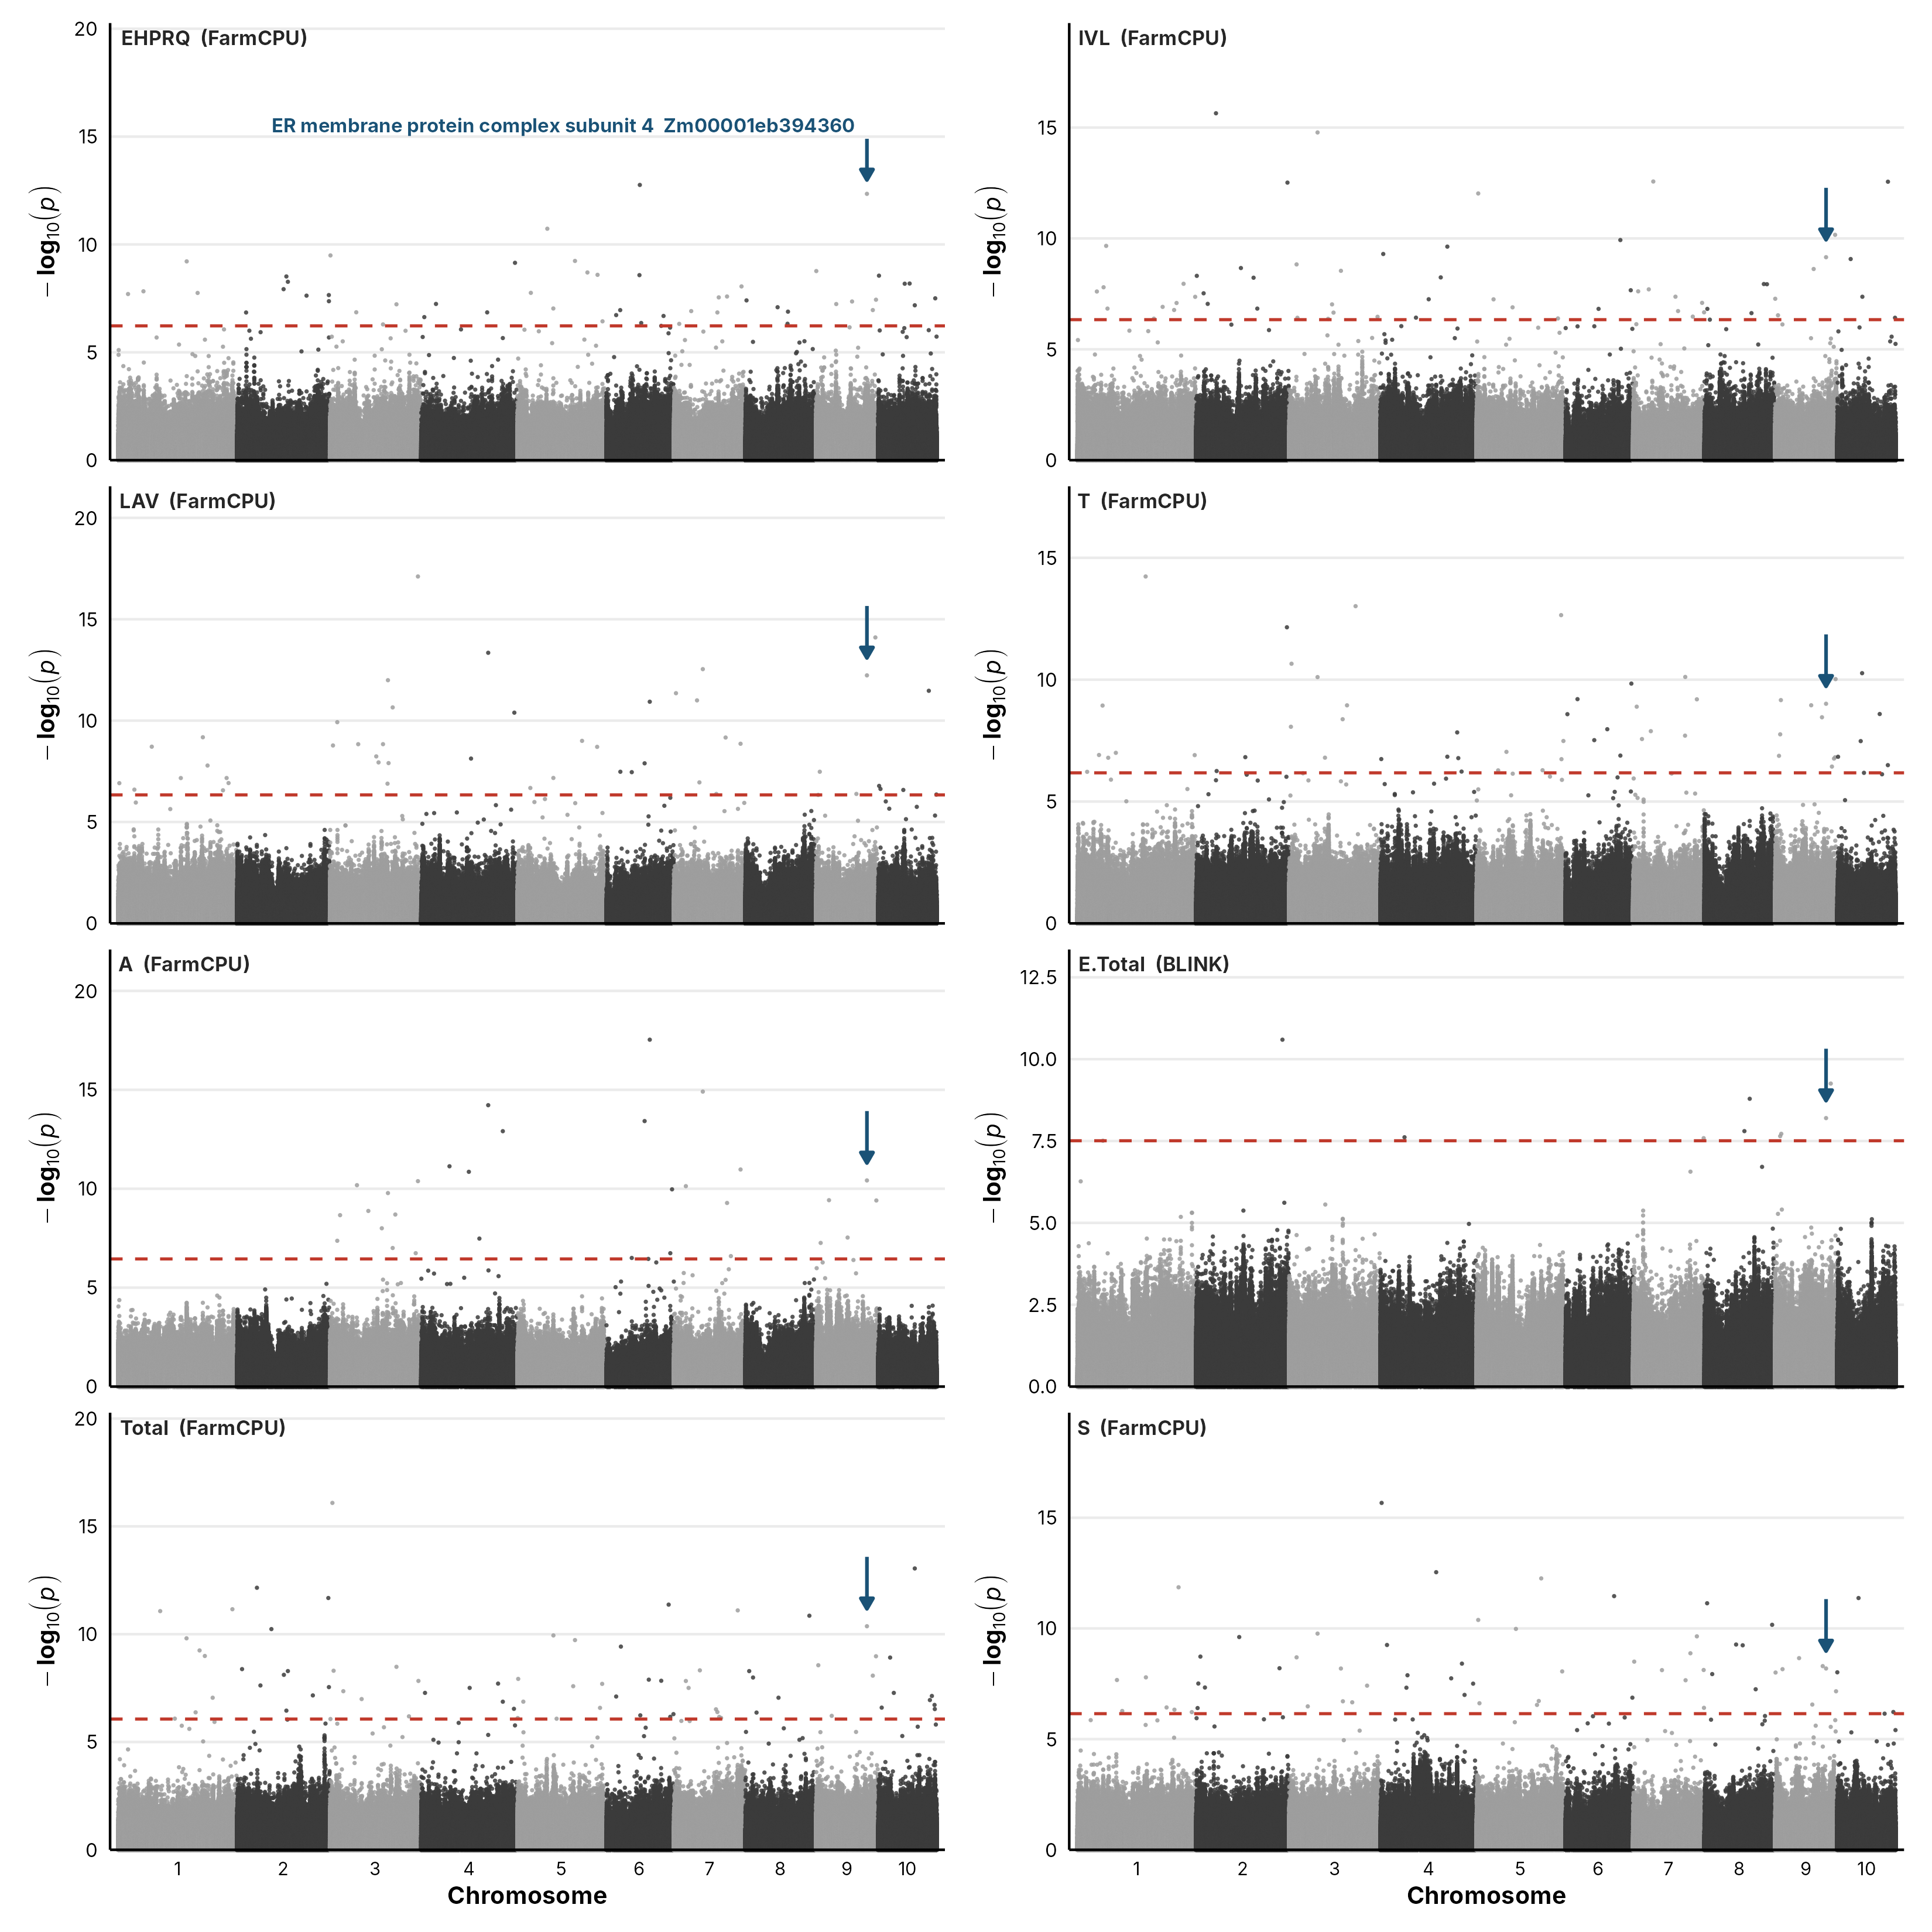
\includegraphics[width=0.82\textwidth]{../supp_figs/SuppFig_amino_chr9_locus_manhattan.png}
\caption*{\textbf{Supplemental Figure S4.} \textbf{Manhattan plots for a locus on chromosome 9 associated with nine amino acid phenotypes.} Eight phenotypes had an FDR-significant association near \textit{Zm00001eb394360} (ER membrane protein complex subunit 4; chr9:133,919,123--133,923,877); \textit{N.E} ($P = 1.1 \times 10^{-7}$) is omitted. Four SNPs spanning 13 kb, from the 3$'$ end of \textit{Zm00001eb394360} to the 5$'$ end of \textit{Zm00001eb394380} (rhomboid-like protein 19), are significant for \textit{A}, \textit{LAV}, \textit{IVL}, \textit{T}, \textit{S}, \textit{Total} and \textit{E.Total}, and two further SNPs are significant for \textit{EHPRQ} and \textit{N.E}. Dashed red lines indicate the 5\% Benjamini--Hochberg FDR threshold. The model for each phenotype is in parentheses.}
\end{figure}
\clearpage

\begin{figure}[p]
\centering
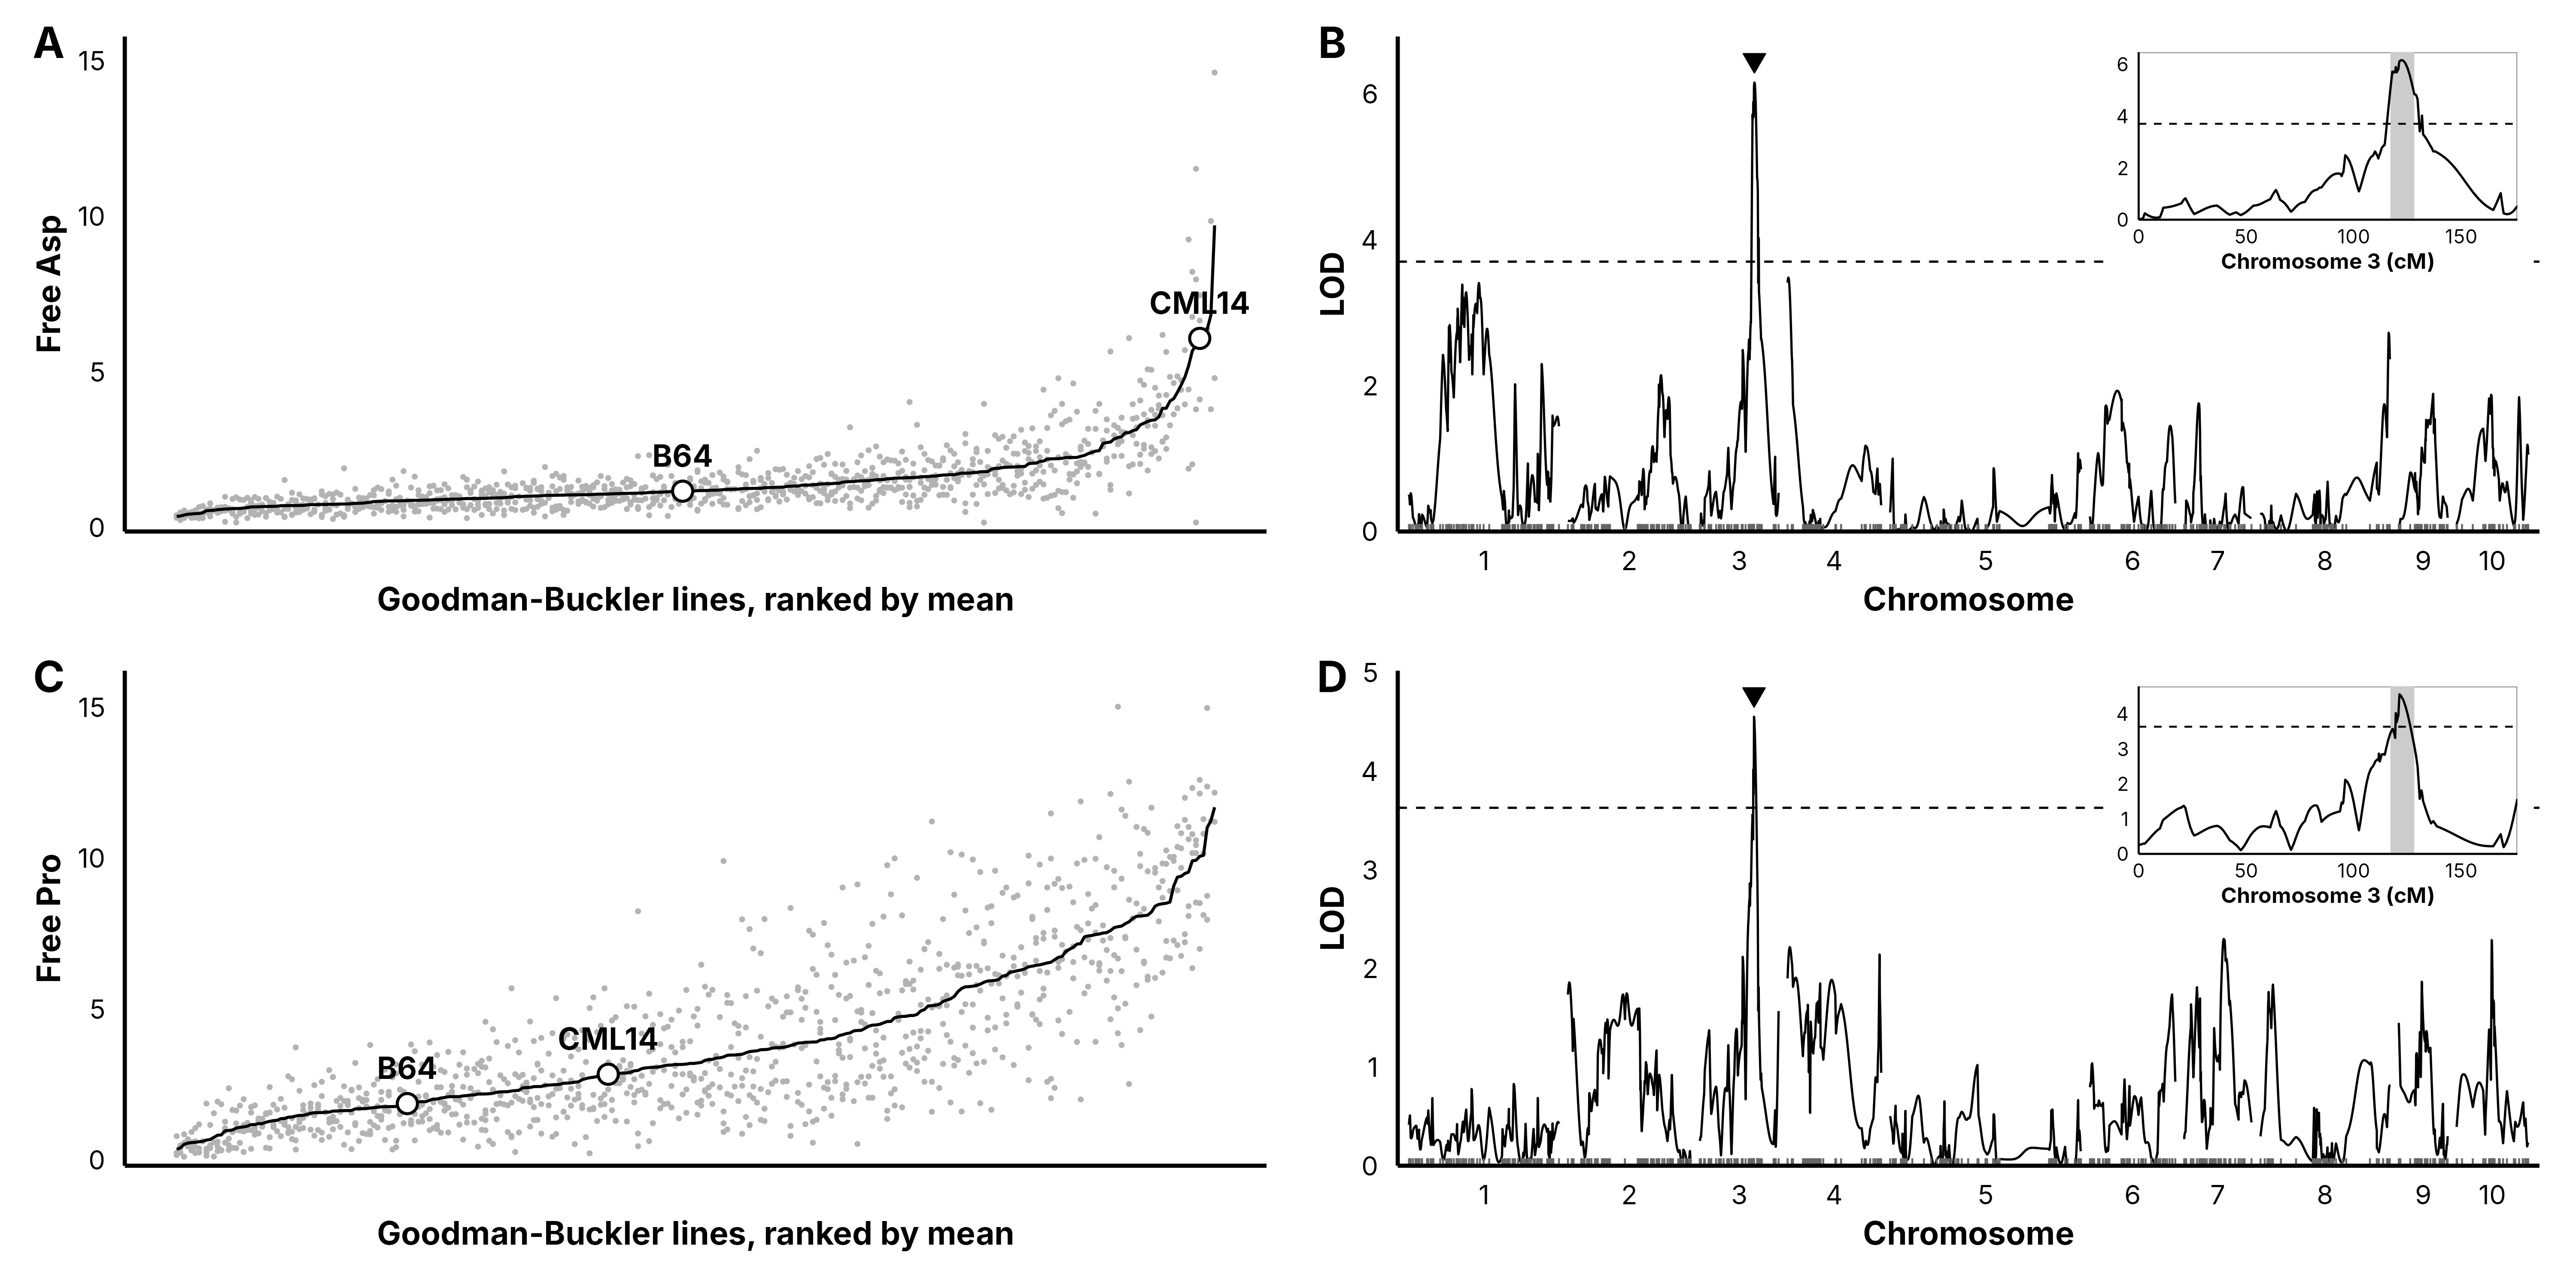
\includegraphics[width=\textwidth]{../supp_figs/SuppFig_QTL_Asp_Pro_panel.png}
\caption*{\textbf{Supplemental Figure S5.} \textbf{Free Asp and Pro map to the same QTL on chromosome 3 in the B64 $\times$ CML14 population.} \textbf{(A, C)} Free Asp (A) and Pro (C) in the Goodman--Buckler panel (nmol~$\mu$g$^{-1}$), with lines ranked by their mean. Open circles mark B64 and CML14. \textbf{(B, D)} Genome-wide LOD scores for free Asp (B) and Pro (D) in the B64 $\times$ CML14 F$_{2:3}$ population. Dashed lines show the genome-wide threshold ($\alpha = 0.05$, 1,000 permutations). The triangle marks the chromosome 3 peak, and the inset shows chromosome 3 with the overlap of the Asp and Pro 1.5-LOD support intervals shaded.}
\end{figure}
\clearpage

\begin{figure}[p]
\centering
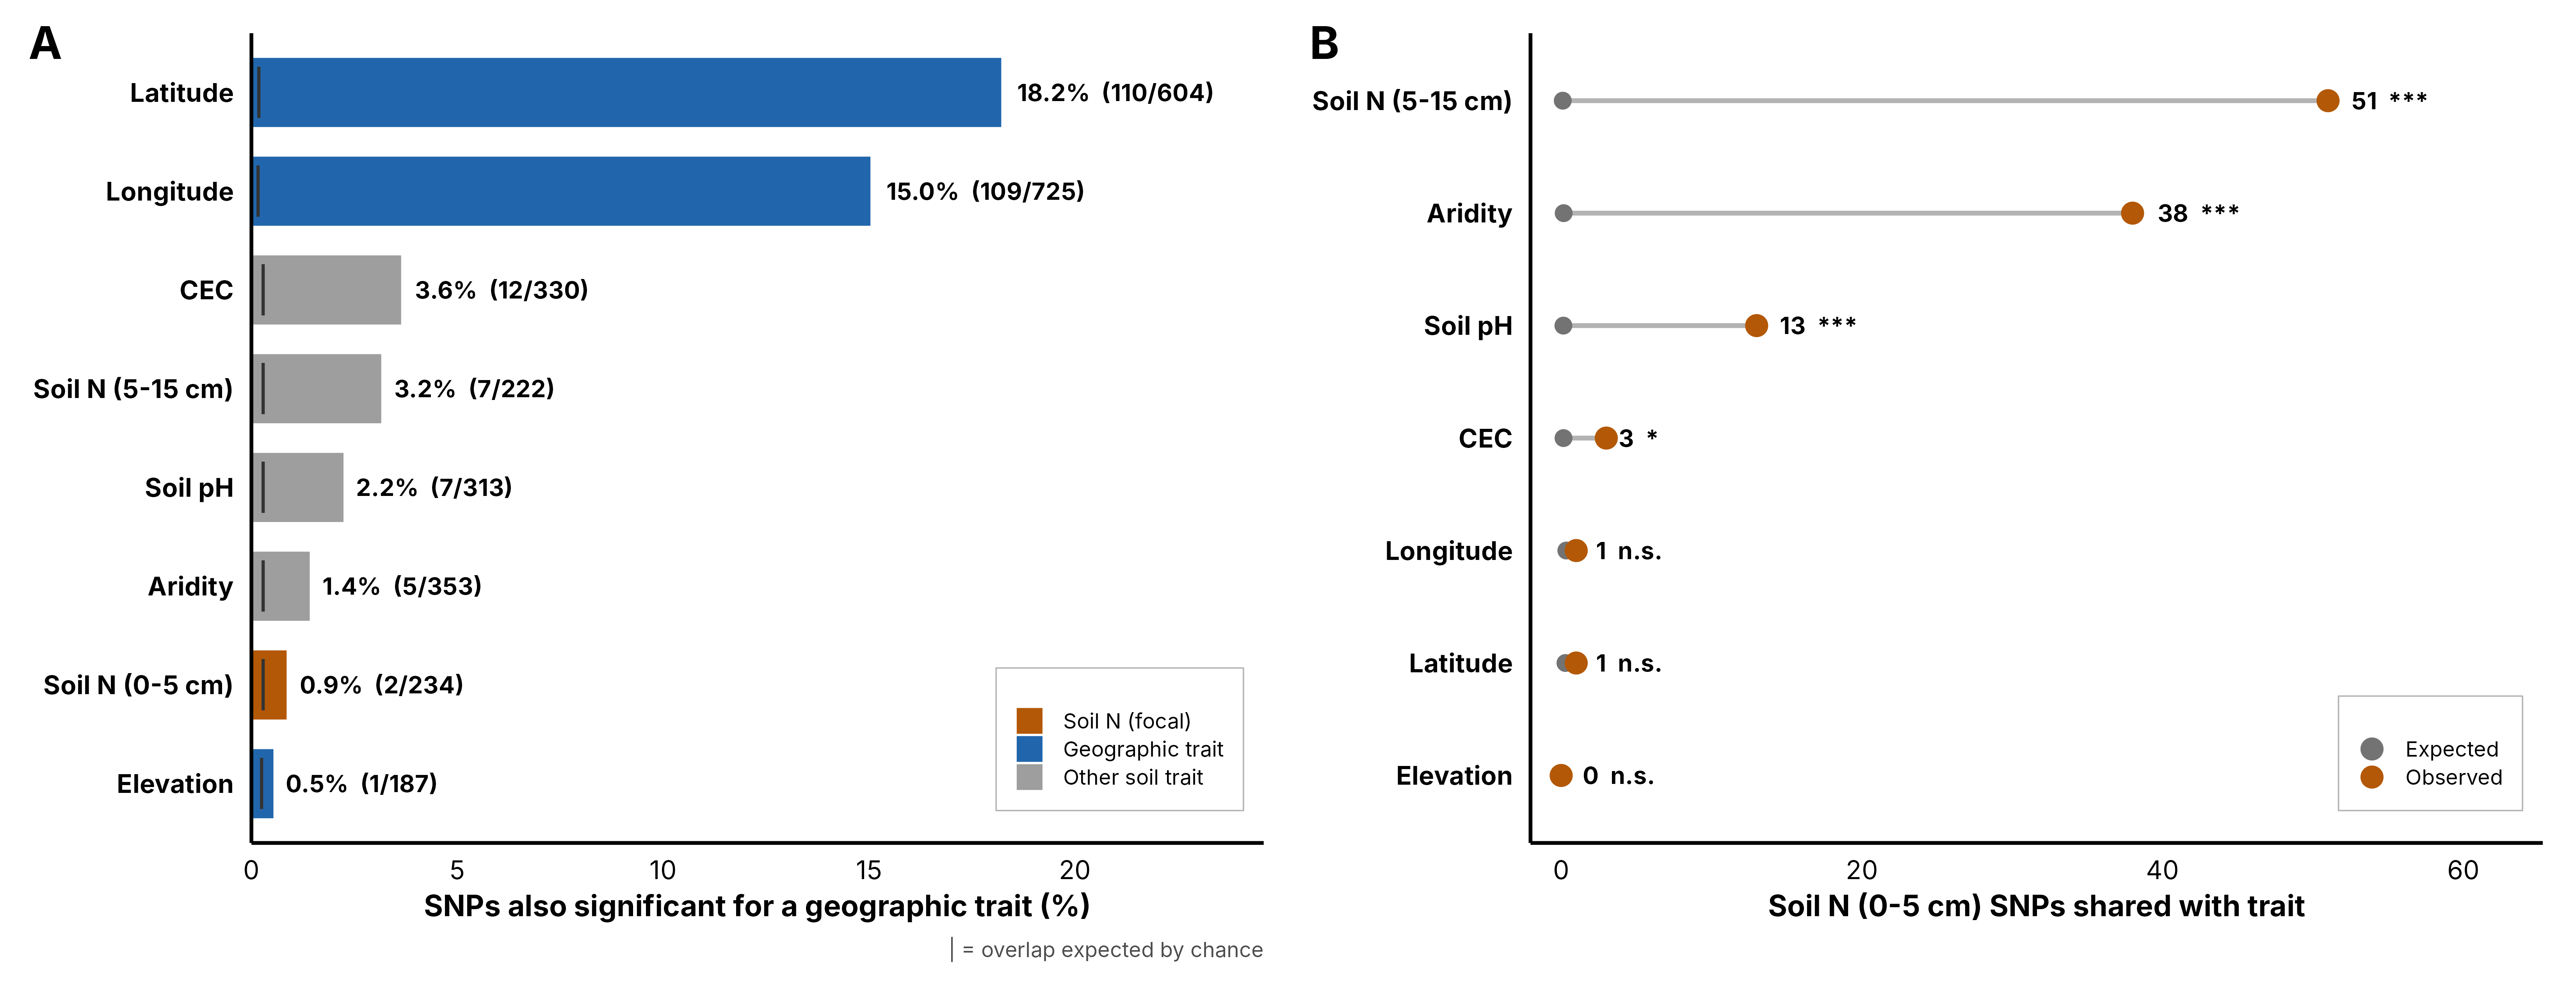
\includegraphics[width=\textwidth]{../supp_figs/SuppFig_soilN_specificity.png}
\caption*{\textbf{Supplemental Figure S6.} \textbf{Overlap of soil-N associations with other environmental GWAS.}
  Each variable was scanned with MLM, BLINK and FarmCPU; a SNP counts as
  significant for a variable if it reaches 5\% FDR in any model.
  \textbf{(A)} Percentage of each variable's significant SNPs that are also significant for a
  geographic variable (latitude, longitude, elevation; the variable itself excluded). Vertical
  ticks, percentage expected by chance.
  \textbf{(B)} SNPs shared between soil N (0--5~cm) and each other variable: observed (orange)
  vs.\ expected (gray). One-sided hypergeometric test, $M = 495{,}755$:
  *\,$P<0.05$; **\,$P<10^{-5}$; ***\,$P<10^{-20}$; n.s., not significant.}
\end{figure}
\clearpage

\begin{figure}[p]
\centering
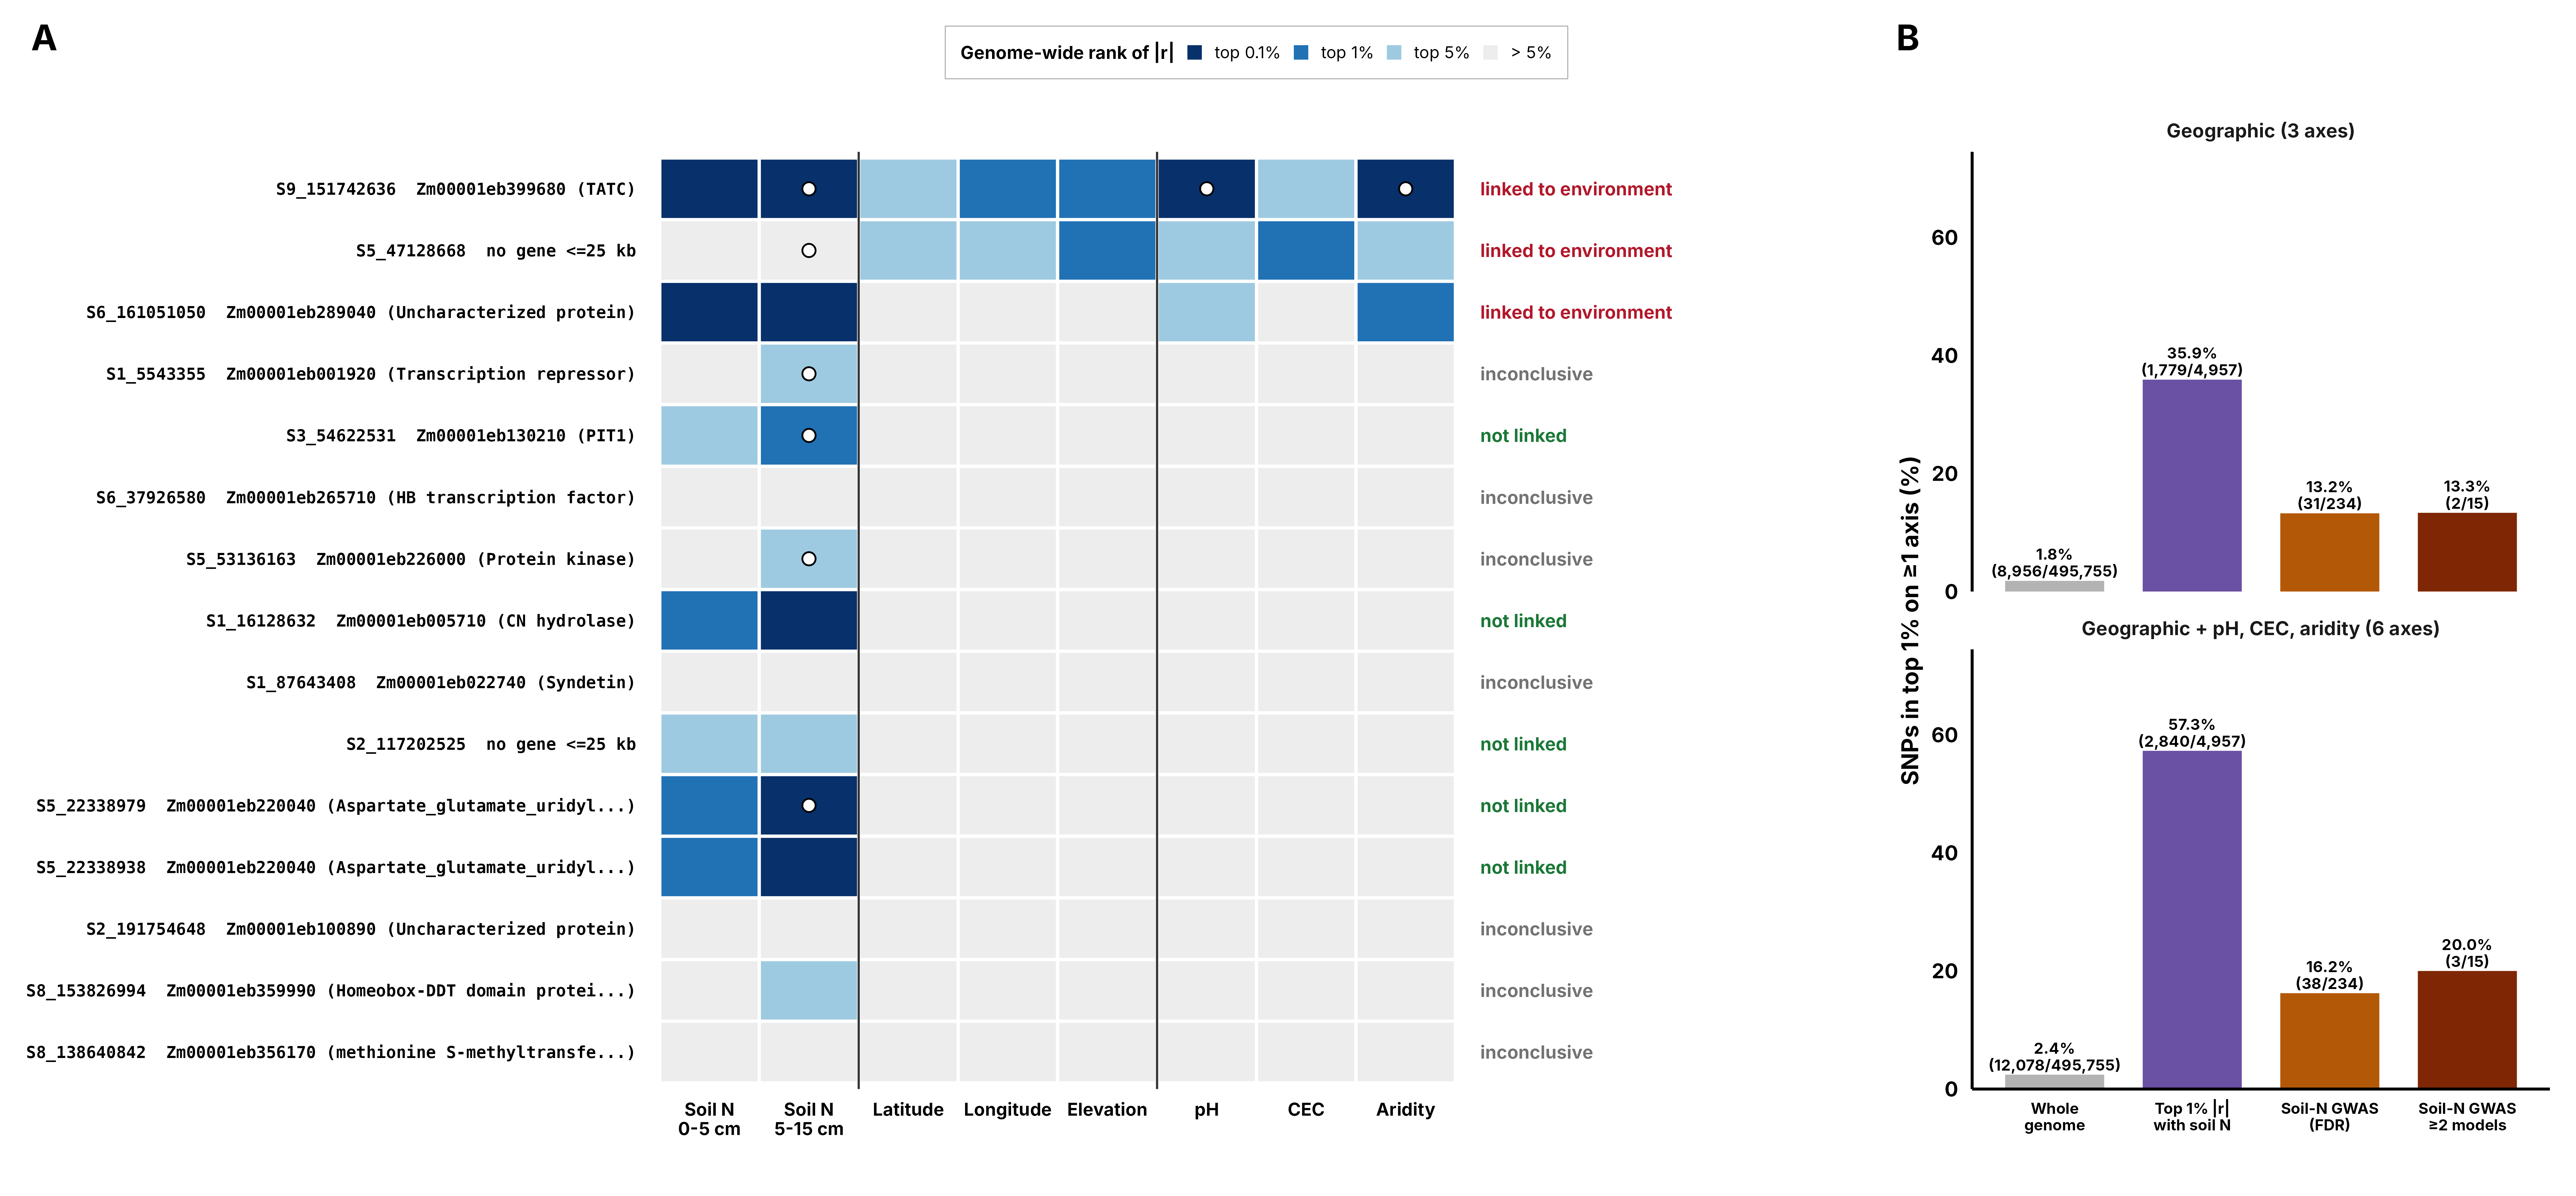
\includegraphics[width=\textwidth]{../supp_figs/SuppFig_soilN_geno_env_correlation.png}
\caption*{\textbf{Supplemental Figure S7.} \textbf{Genotype--environment correlation test for the soil-N SNPs.}
  We computed the Pearson correlation ($r$) between the SNP's genotype
  (0, 1 or 2 copies of the allele) and each site variable across 3,107 accessions, then ranked
  every SNP against the whole genome by $|r|$ (e.g.\ ``top 1\%'' = fewer than 1\% of SNPs
  correlate more strongly with that variable).
  \textbf{(A)} The 15 soil-N SNPs significant in at least two GWAS models. Tile color shows the
  genome-wide rank of each SNP's correlation with each variable. Open circles mark SNPs that were
  also significant (5\% FDR) in that variable's own GWAS. Each SNP's call is shown on the right:
  \textit{linked to environment}, its genotype is in the top 1\% of the genome for correlation
  with at least one non-N variable, so its soil-N association cannot be separated from geography
  or climate;
  \textit{not linked}, its genotype correlates strongly with soil N (top 5\%) but not with any
  other variable;
  \textit{inconclusive}, its genotype correlates only weakly with soil N across all accessions
  (outside the top 5\%), so there is no soil-N correlation to compare the other variables
  against. These SNPs were detected only by BLINK and FarmCPU, which test each SNP after
  accounting for population structure and other strongly associated SNPs; this test applies no
  such adjustment and therefore cannot judge them in either direction.
  \textbf{(B)} Expectation test: percentage of SNPs whose genotype is in the top 1\% for at least
  one geographic variable (latitude, longitude, elevation; top) or for at least one of all six
  non-N variables (bottom), for the whole genome, for SNPs in the top 1\% for correlation with
  soil N, and for the soil-N GWAS SNPs.}
\end{figure}
\clearpage

\begin{figure}[p]
\centering
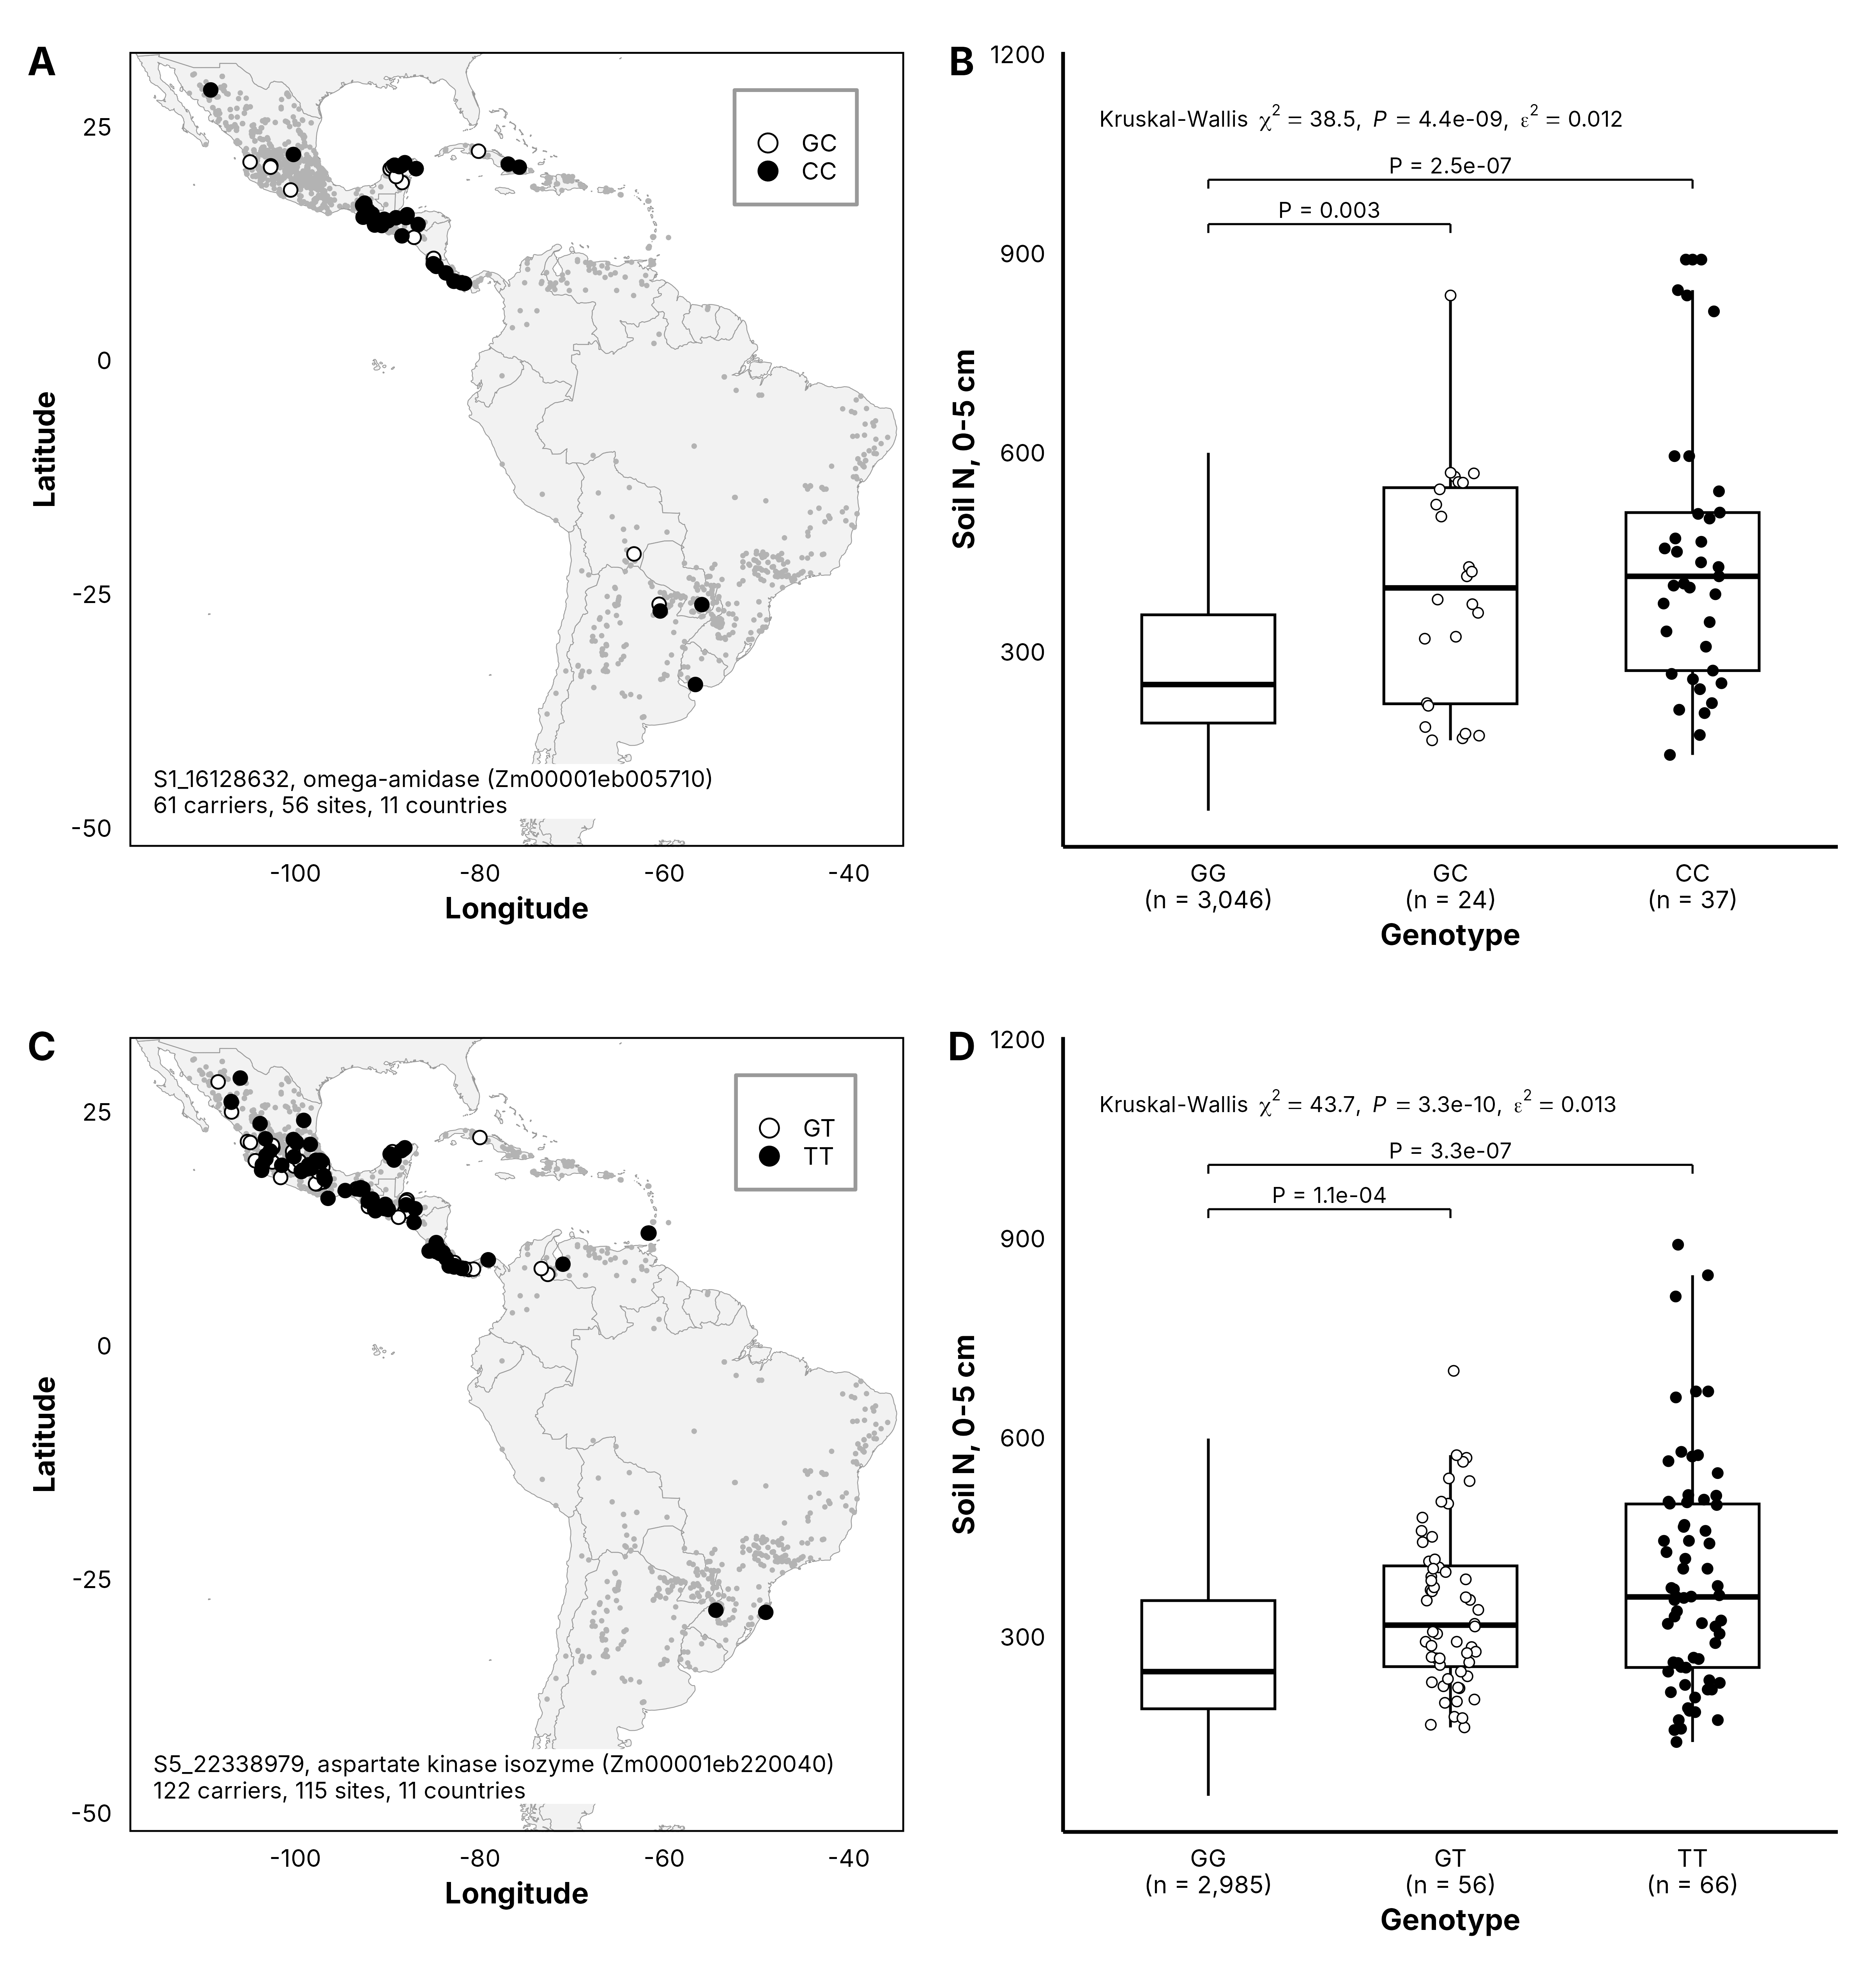
\includegraphics[width=0.85\textwidth]{../supp_figs/SuppFig_soilN_focal_allele_geography.png}
\caption*{\textbf{Supplemental Figure S8.} \textbf{Geography and soil N of the two focal soil-N SNPs.} \textbf{(A, B)} S1\_16128632 in the $\omega$-amidase gene \textit{Zm00001eb005710}. \textbf{(C, D)} S5\_22338979 near the aspartate kinase isozyme gene \textit{Zm00001eb220040}. \textbf{(A, C)} Collection sites of the 3,107 landraces. Gray, homozygous for the major allele; white, heterozygous; black, homozygous for the minor allele. Numbers of carriers, independent collection sites, and countries are given in each panel. \textbf{(B, D)} Soil N at 0--5 cm by genotype. Boxes show the median and interquartile range, and points show individual values. Differences among genotypes were tested with a Kruskal--Wallis test ($\varepsilon^2$, effect size), followed by Dunn tests with Holm correction, and only significant pairwise comparisons are shown.}
\end{figure}
\clearpage

\begin{figure}[p]
\centering
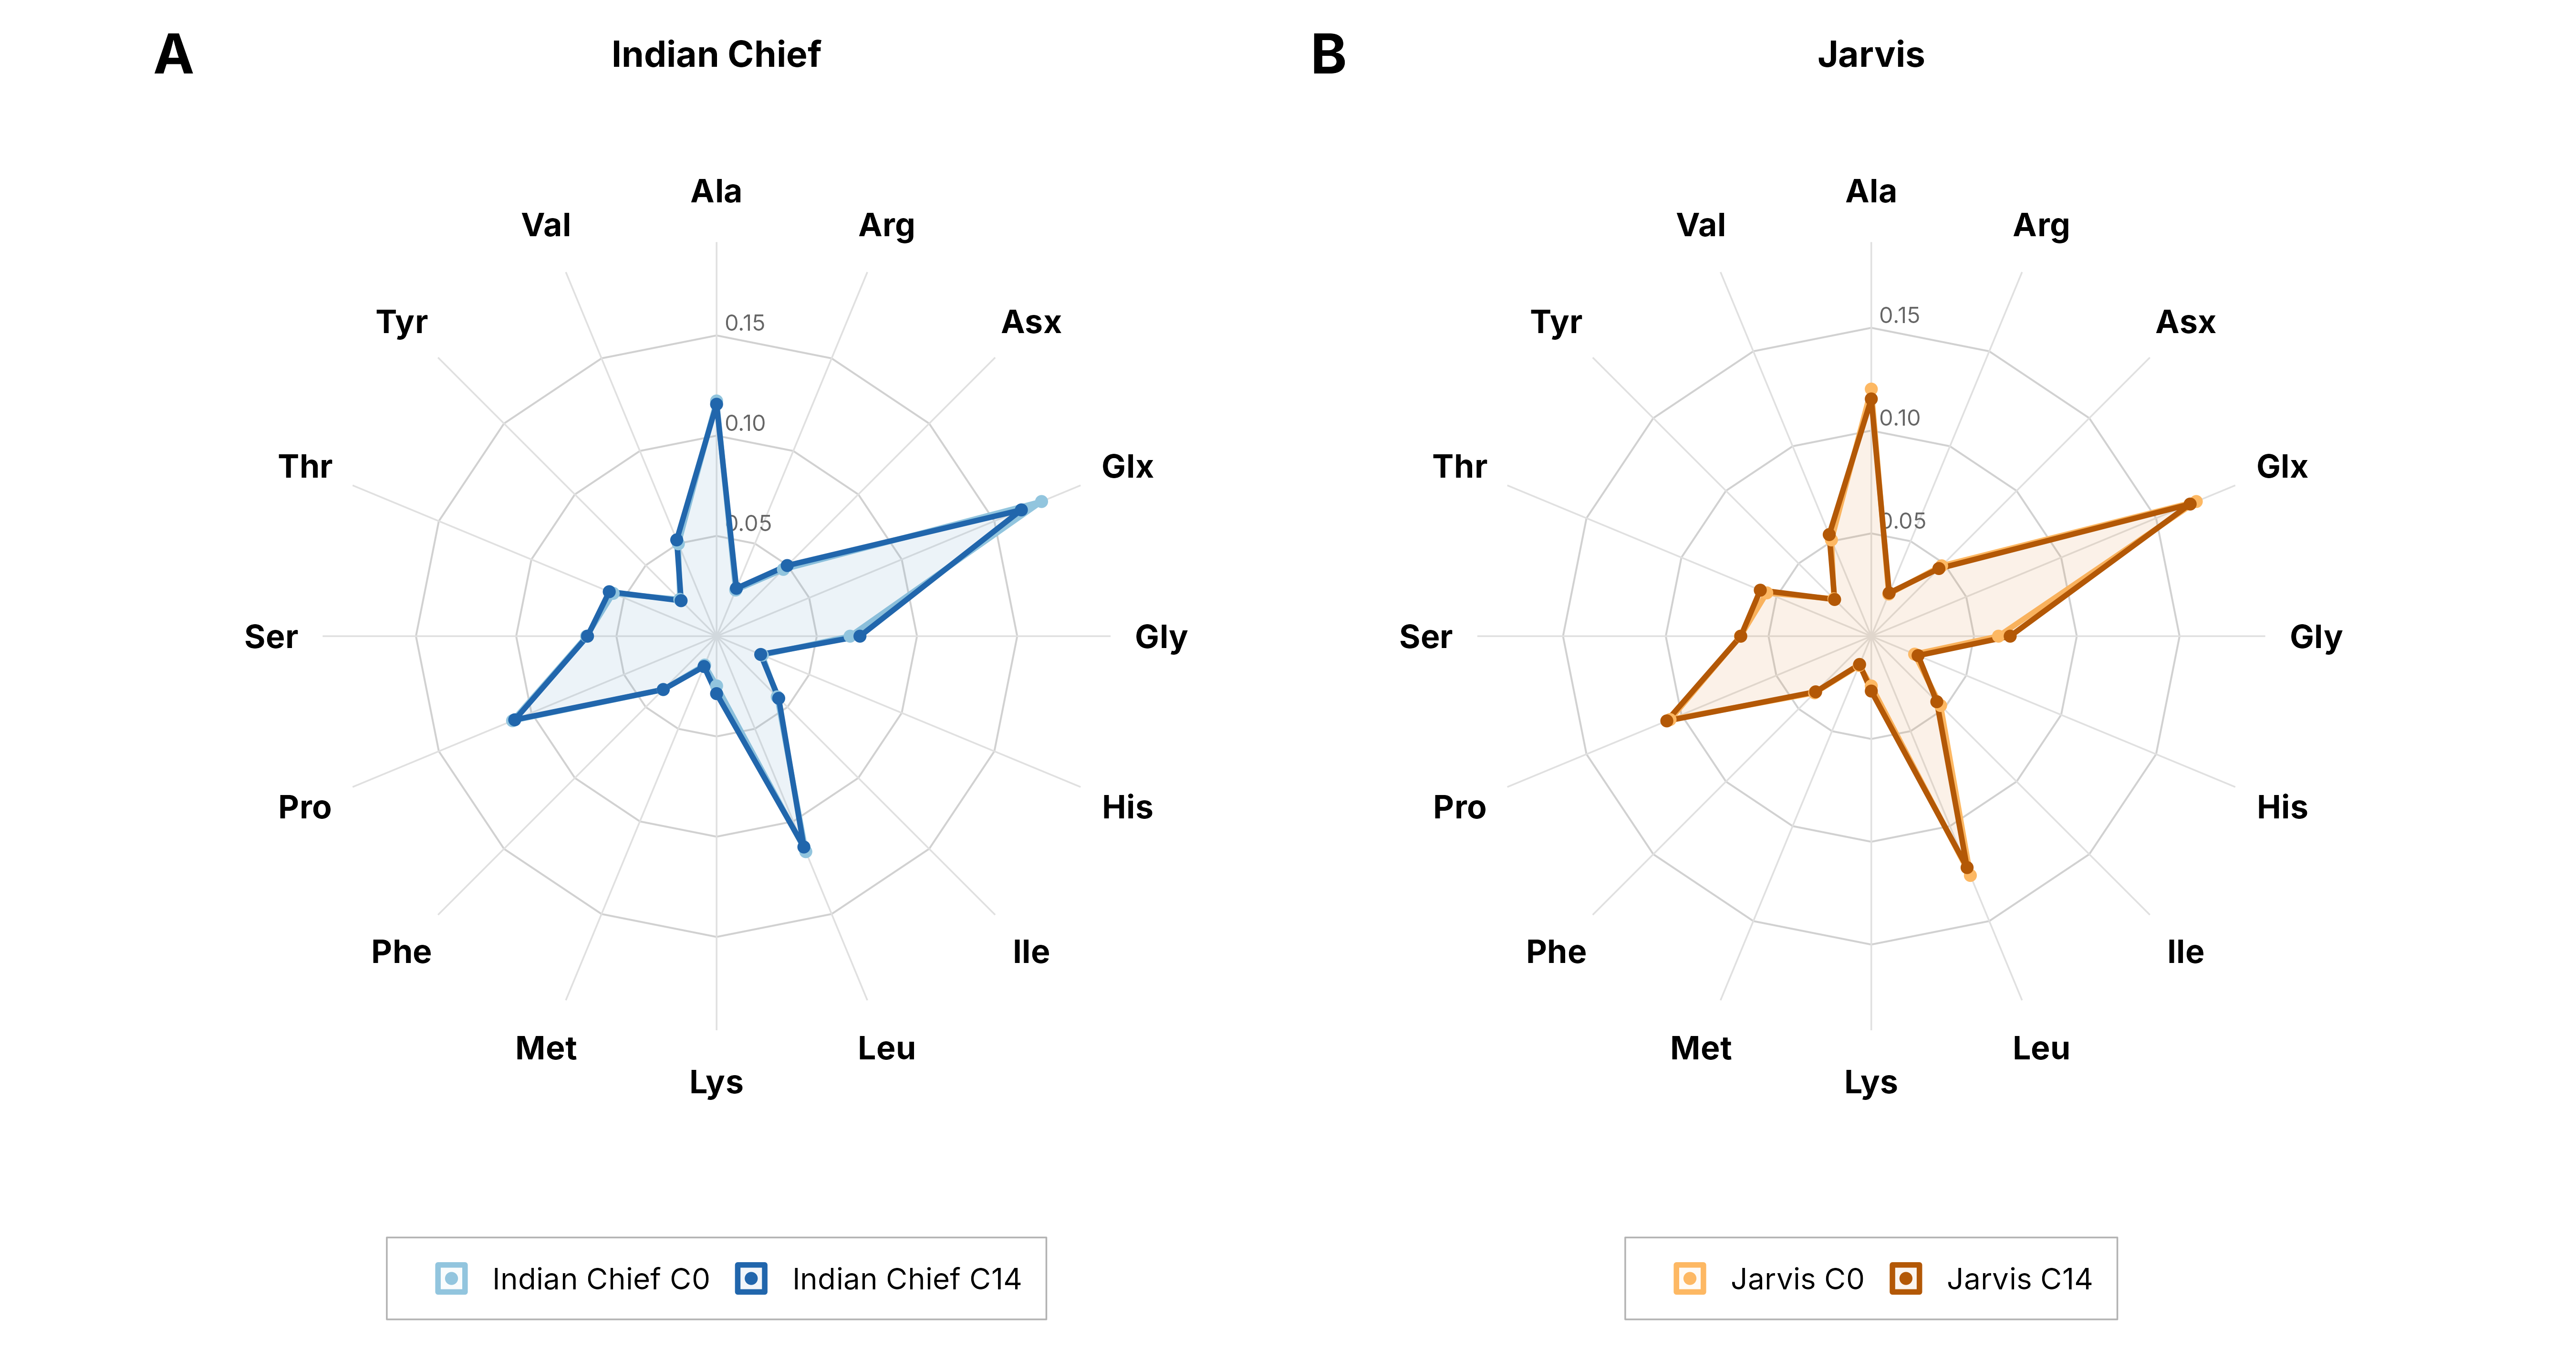
\includegraphics[width=\textwidth]{../supp_figs/SuppFig_IC_J_PBAA_composition.png}
\caption*{\textbf{Supplemental Figure S9.} \textbf{Protein-bound amino acid (PBAA) composition in Indian Chief and Jarvis at Cycle 0 (C0) and Cycle 14 (C14).} Mean fraction of each of 16 PBAA in the total PBAA pool, averaged over biological samples, for \textbf{(A)} Indian Chief and \textbf{(B)} Jarvis. Asx and Glx are the combined Asp + Asn and Glu + Gln pools after acid hydrolysis; tryptophan and cysteine are not measured. Rings mark fractions of 0.05, 0.10 and 0.15. No amino acid differed between cycles in either population (two-sided Wilcoxon rank-sum tests, Benjamini--Hochberg-adjusted across the 16 amino acids.}
\end{figure}
\clearpage

\begin{figure}[p]
\centering
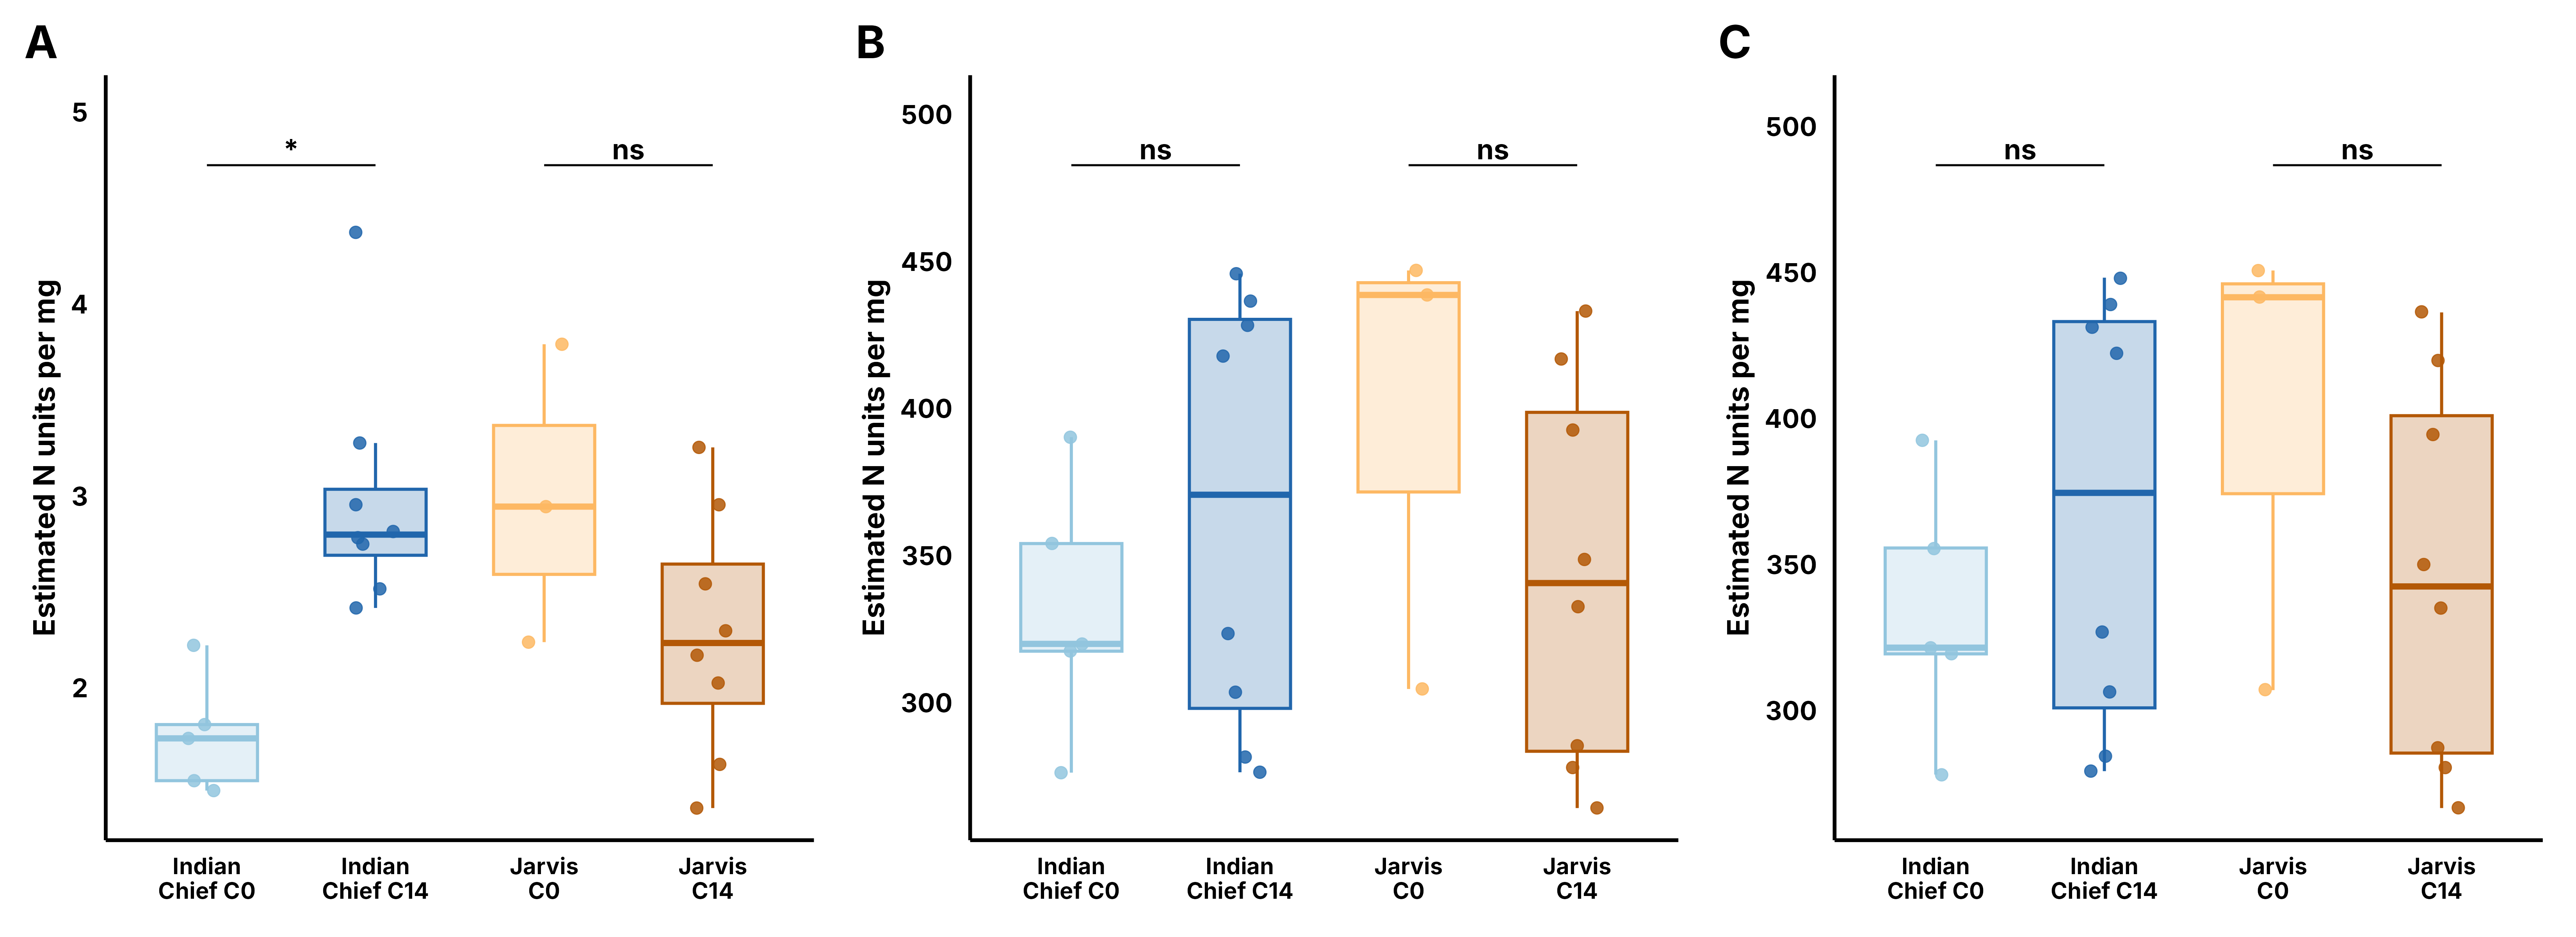
\includegraphics[width=\textwidth]{../supp_figs/SuppFig_IC_J_AA_N_pools.png}
\caption*{\textbf{Supplemental Figure S10.} \textbf{Amino acid-derived nitrogen per mg sample in Indian Chief and Jarvis at Cycle 0 (C0) and Cycle~14 (C14).} \textbf{(A)} FAA-derived N, \textbf{(B)} estimated protein-bound amino acid-derived N and \textbf{(C)} estimated total amino acid-derived N (A + B). Each amino acid was weighted by its number of N atoms (Arg 4; His 3; Asn, Gln, Lys and Trp 2; all others 1; protein-bound Asx and Glx 1.5) and divided by sample mass. Points are biological samples (Indian Chief C0 $n = 5$, C14 $n = 8$; Jarvis C0 $n = 3$, C14 $n = 8$); boxes show the median and interquartile range. Brackets show within-population two-sided Wilcoxon rank-sum tests, Benjamini--Hochberg-adjusted across the three measures: * adjusted $P < 0.05$; ns, not significant.}
\end{figure}
\clearpage

\begin{figure}[p]
\centering
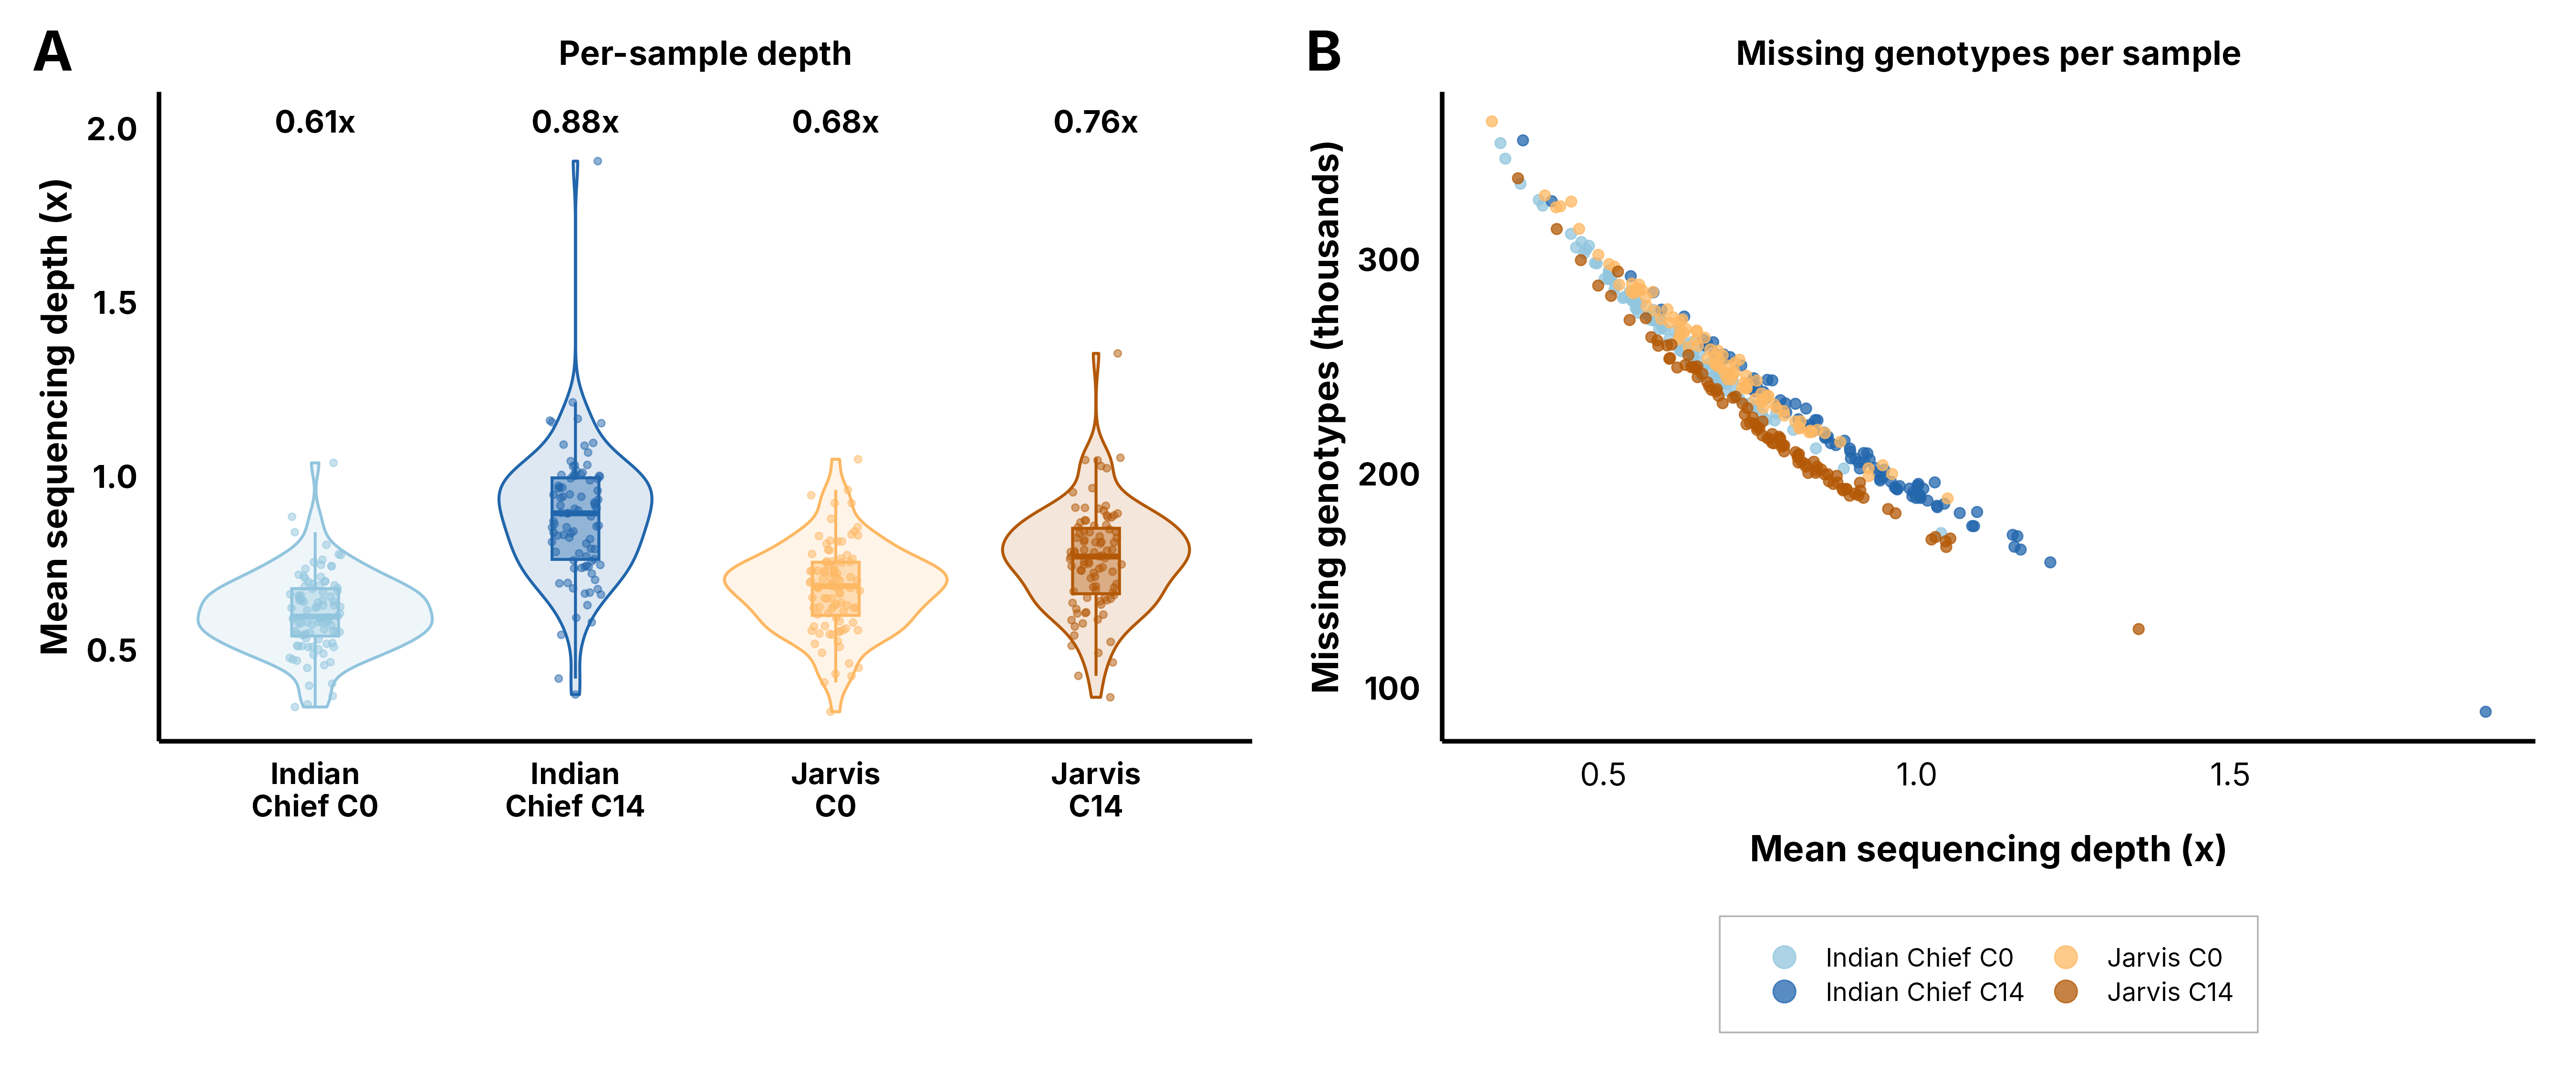
\includegraphics[width=\textwidth]{../supp_figs/SuppFig_seq_statistics_sample_level.png}
\caption*{\textbf{Supplemental Figure S11.} \textbf{Per-sample sequencing depth in the Indian Chief and Jarvis skim-sequencing data.} \textbf{(A)} Mean sequencing depth per individual for each population and cycle; numbers give group means. \textbf{(B)} Number of missing genotypes (of 512,667 filtered SNPs) per individual against its mean depth.}
\end{figure}
\clearpage

\begin{figure}[p]
\centering
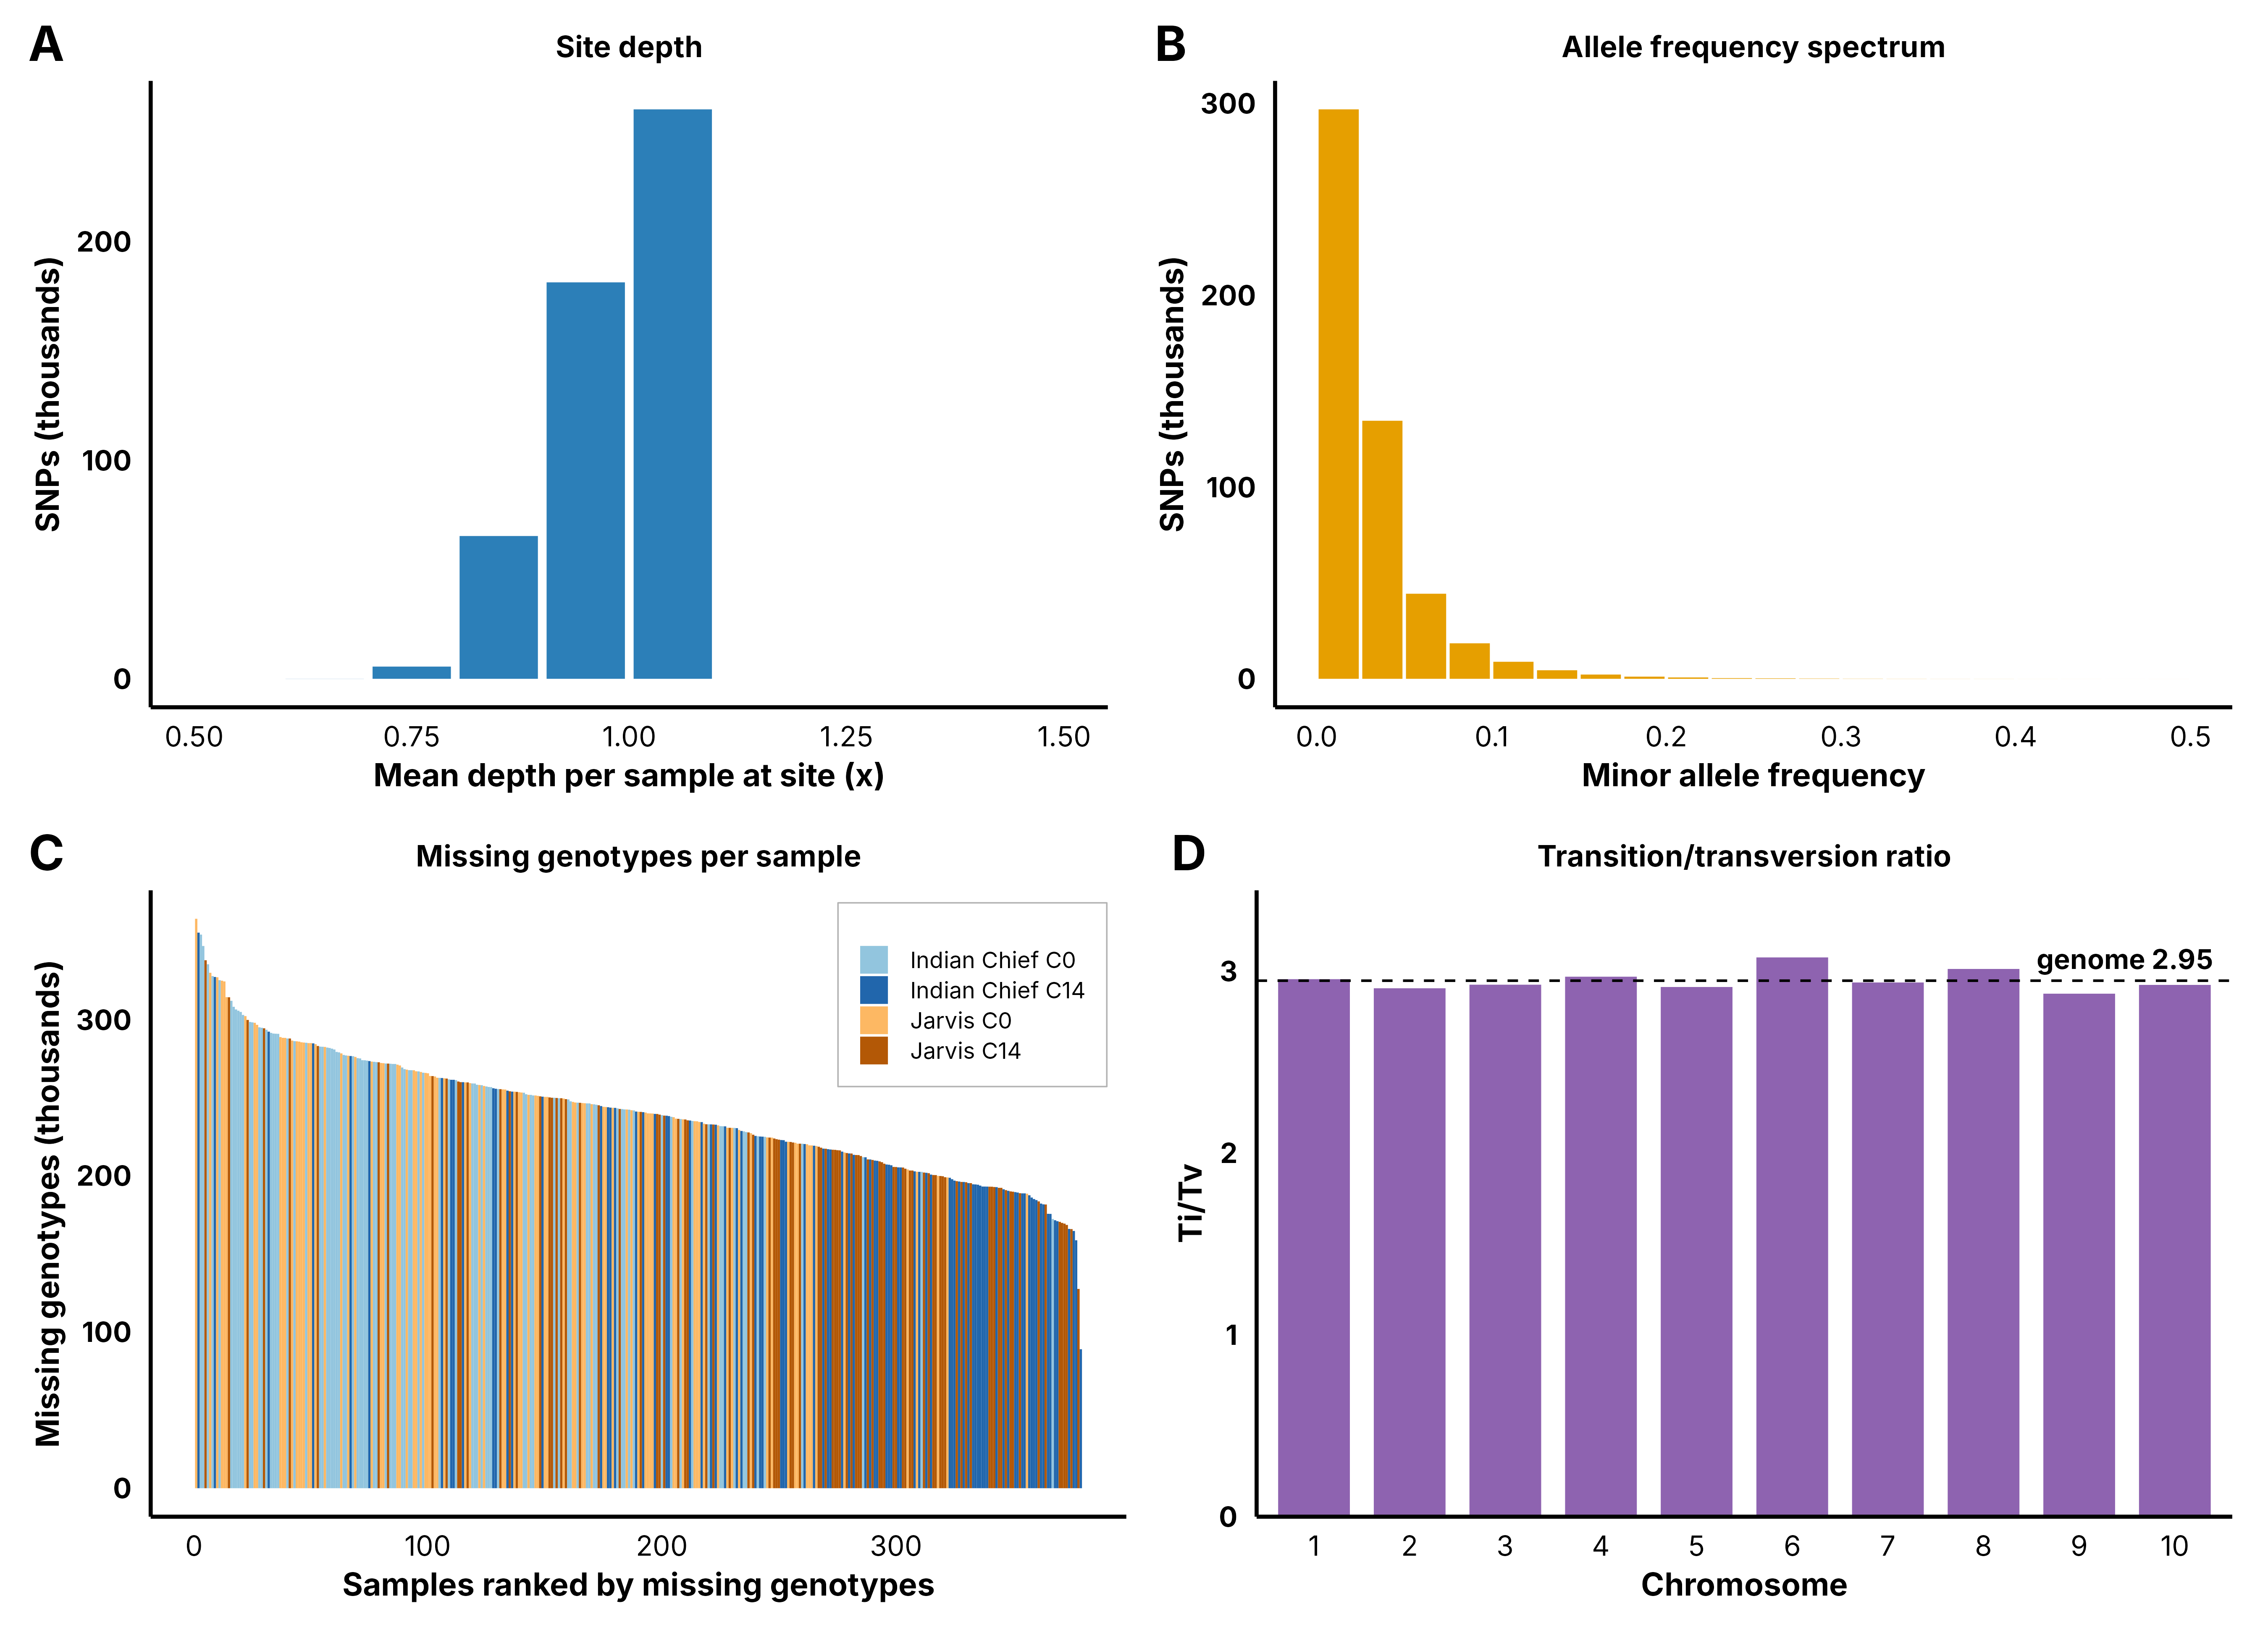
\includegraphics[width=\textwidth]{../supp_figs/SuppFig_seq_statistics_variant_level.png}
\caption*{\textbf{Supplemental Figure S12.} \textbf{Quality summaries for the 512,667 filtered SNPs.} \textbf{(A)} Mean depth per individual at each SNP (total site depth divided by 379). \textbf{(B)} Minor allele frequency spectrum, from called genotypes. \textbf{(C)} Missing genotypes per individual, ranked and colored by population and cycle. \textbf{(D)} Transition/transversion ratio by chromosome; dashed line, genome-wide value.}
\end{figure}
\clearpage

\begin{figure}[p]
\centering
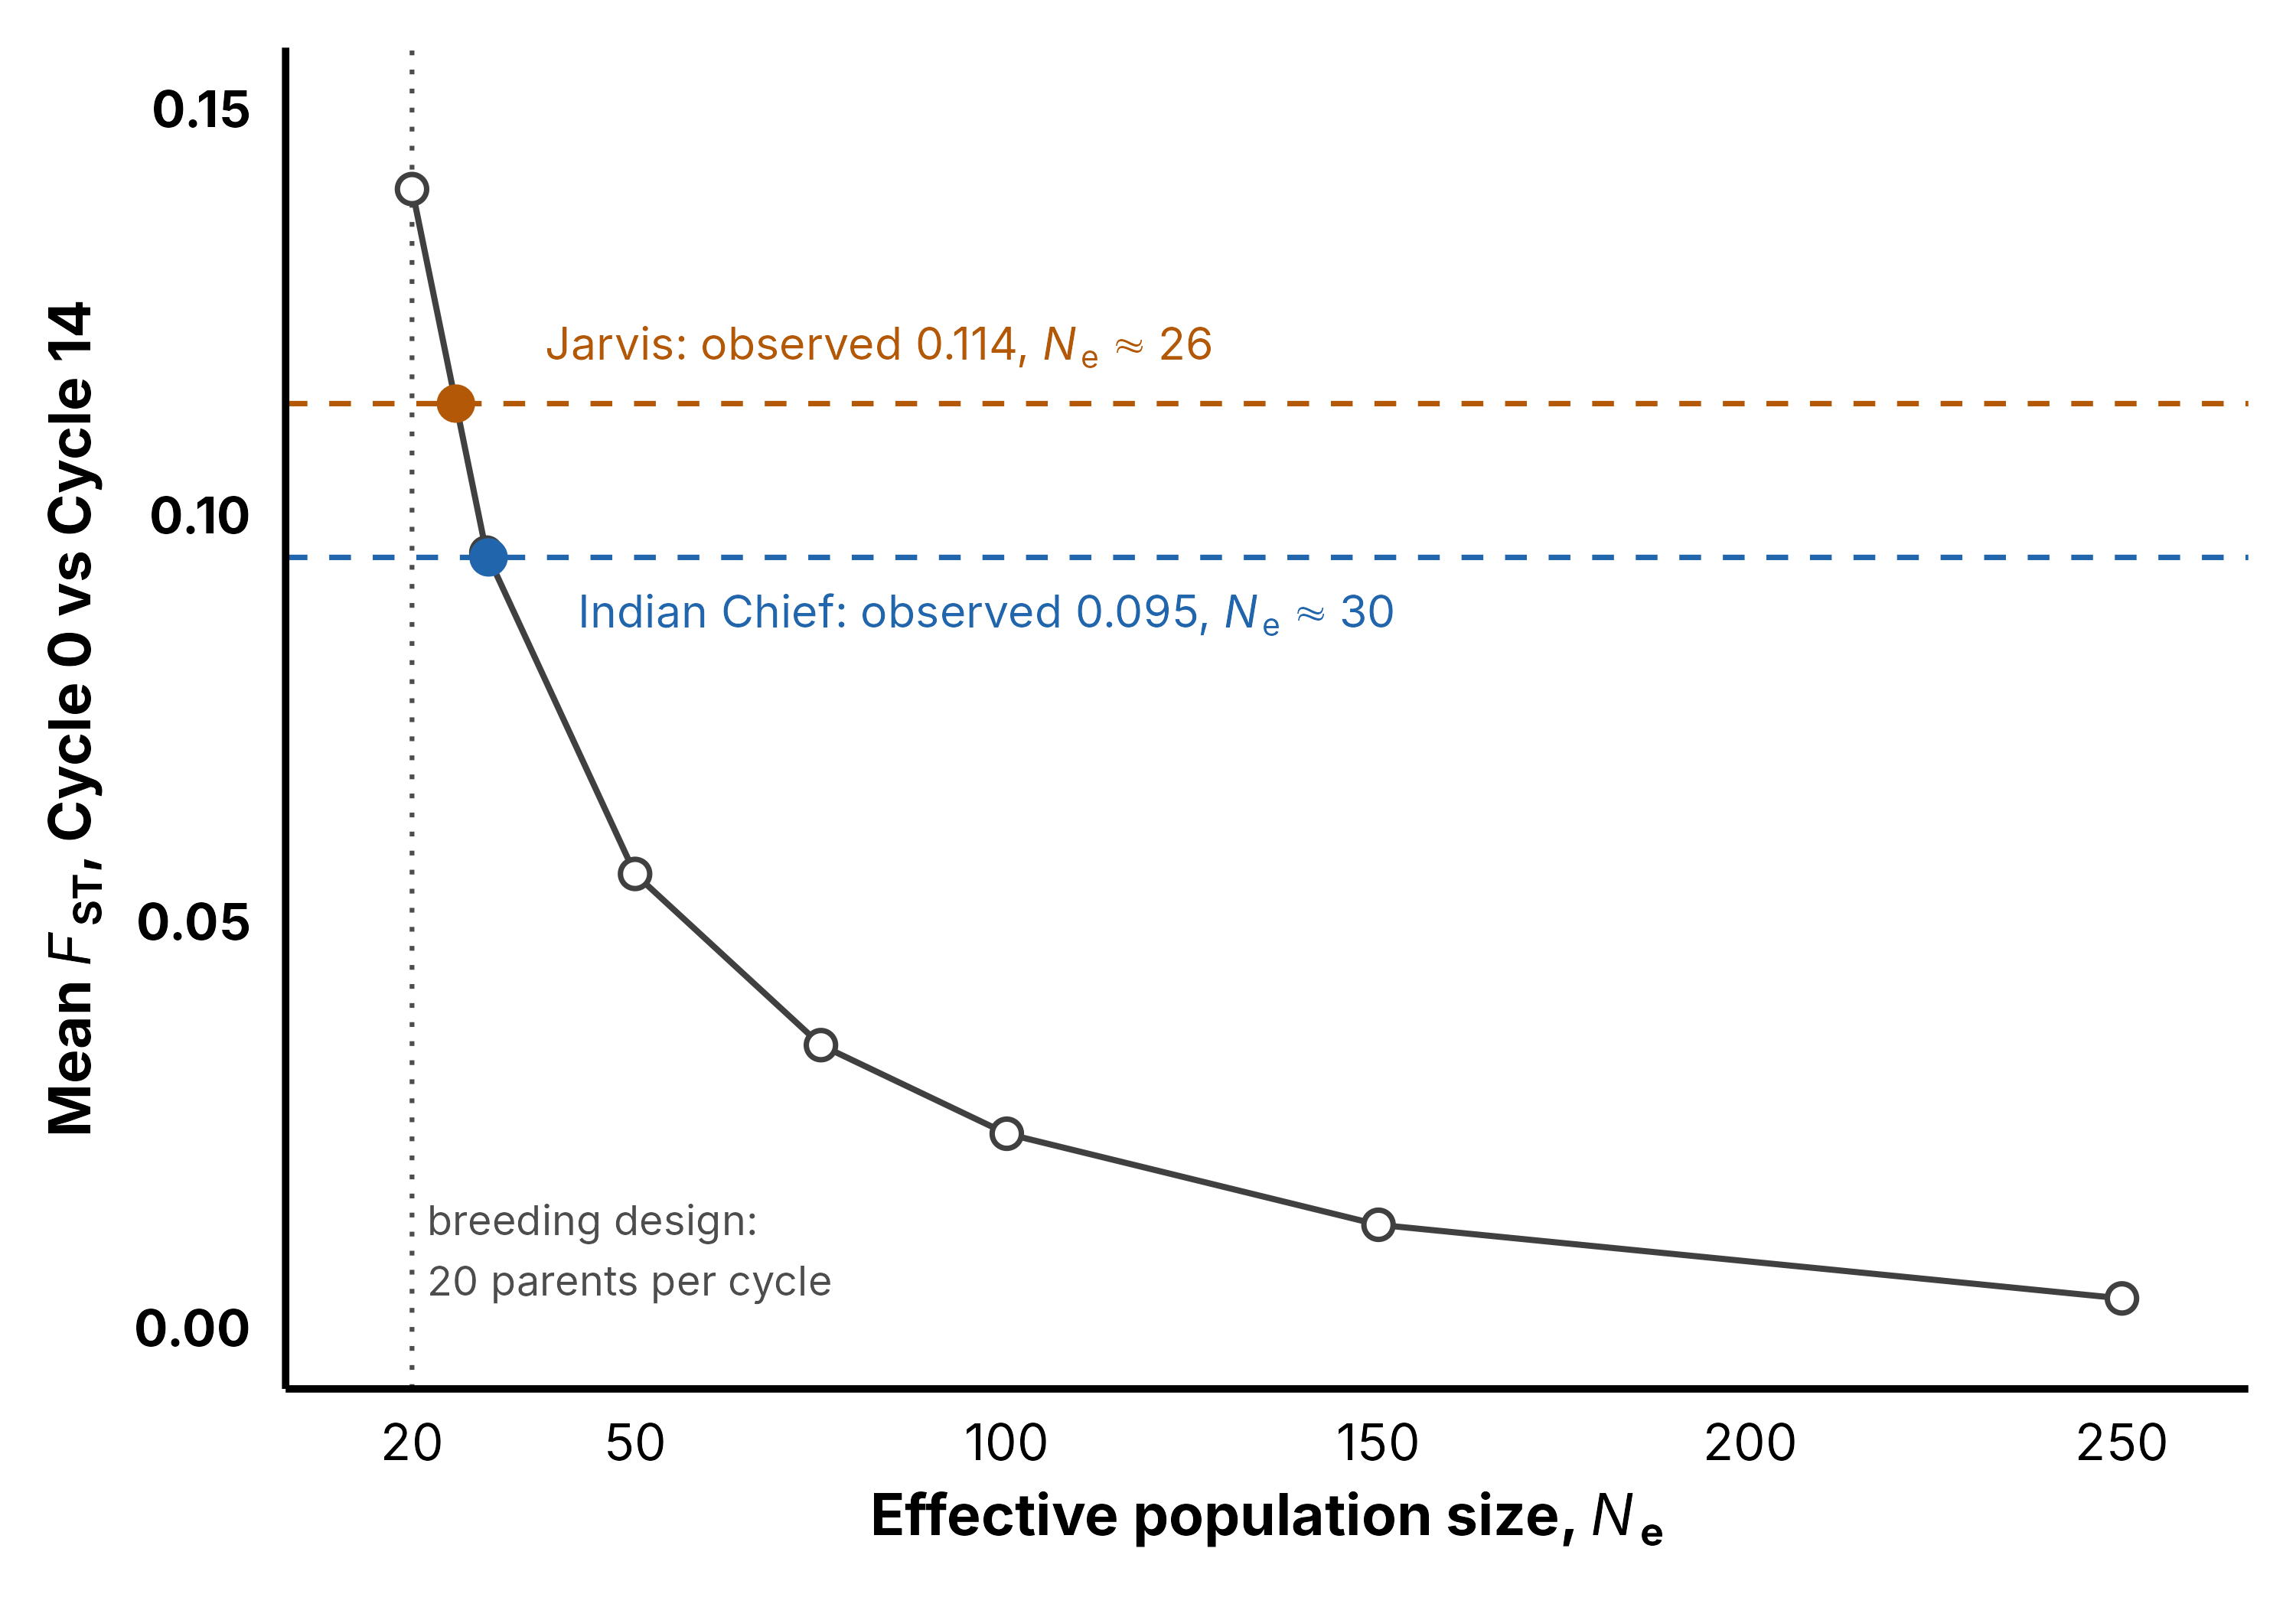
\includegraphics[width=0.75\textwidth]{../supp_figs/SuppFig_IC_J_Ne_drift.png}
\caption*{\textbf{Supplemental Figure S13.} \textbf{Effective population size of the Indian Chief and Jarvis recurrent-selection populations.} Genome-wide mean $F_{ST}$ between Cycle~0 and Cycle~14 expected under neutral Wright--Fisher drift for 14 generations across a range of effective population sizes ($N_e$; open circles), starting from the observed Cycle~0 allele frequencies and resampling the number of individuals sequenced at each site. Dashed lines give the observed values (Indian Chief 0.095, Jarvis 0.114), and filled circles mark the implied $N_e$, obtained by linear interpolation. The dotted line marks $N_e = 20$, the value expected when the 20 parents intermated in each cycle contribute equally.}
\end{figure}
\clearpage

\begin{figure}[p]
\centering
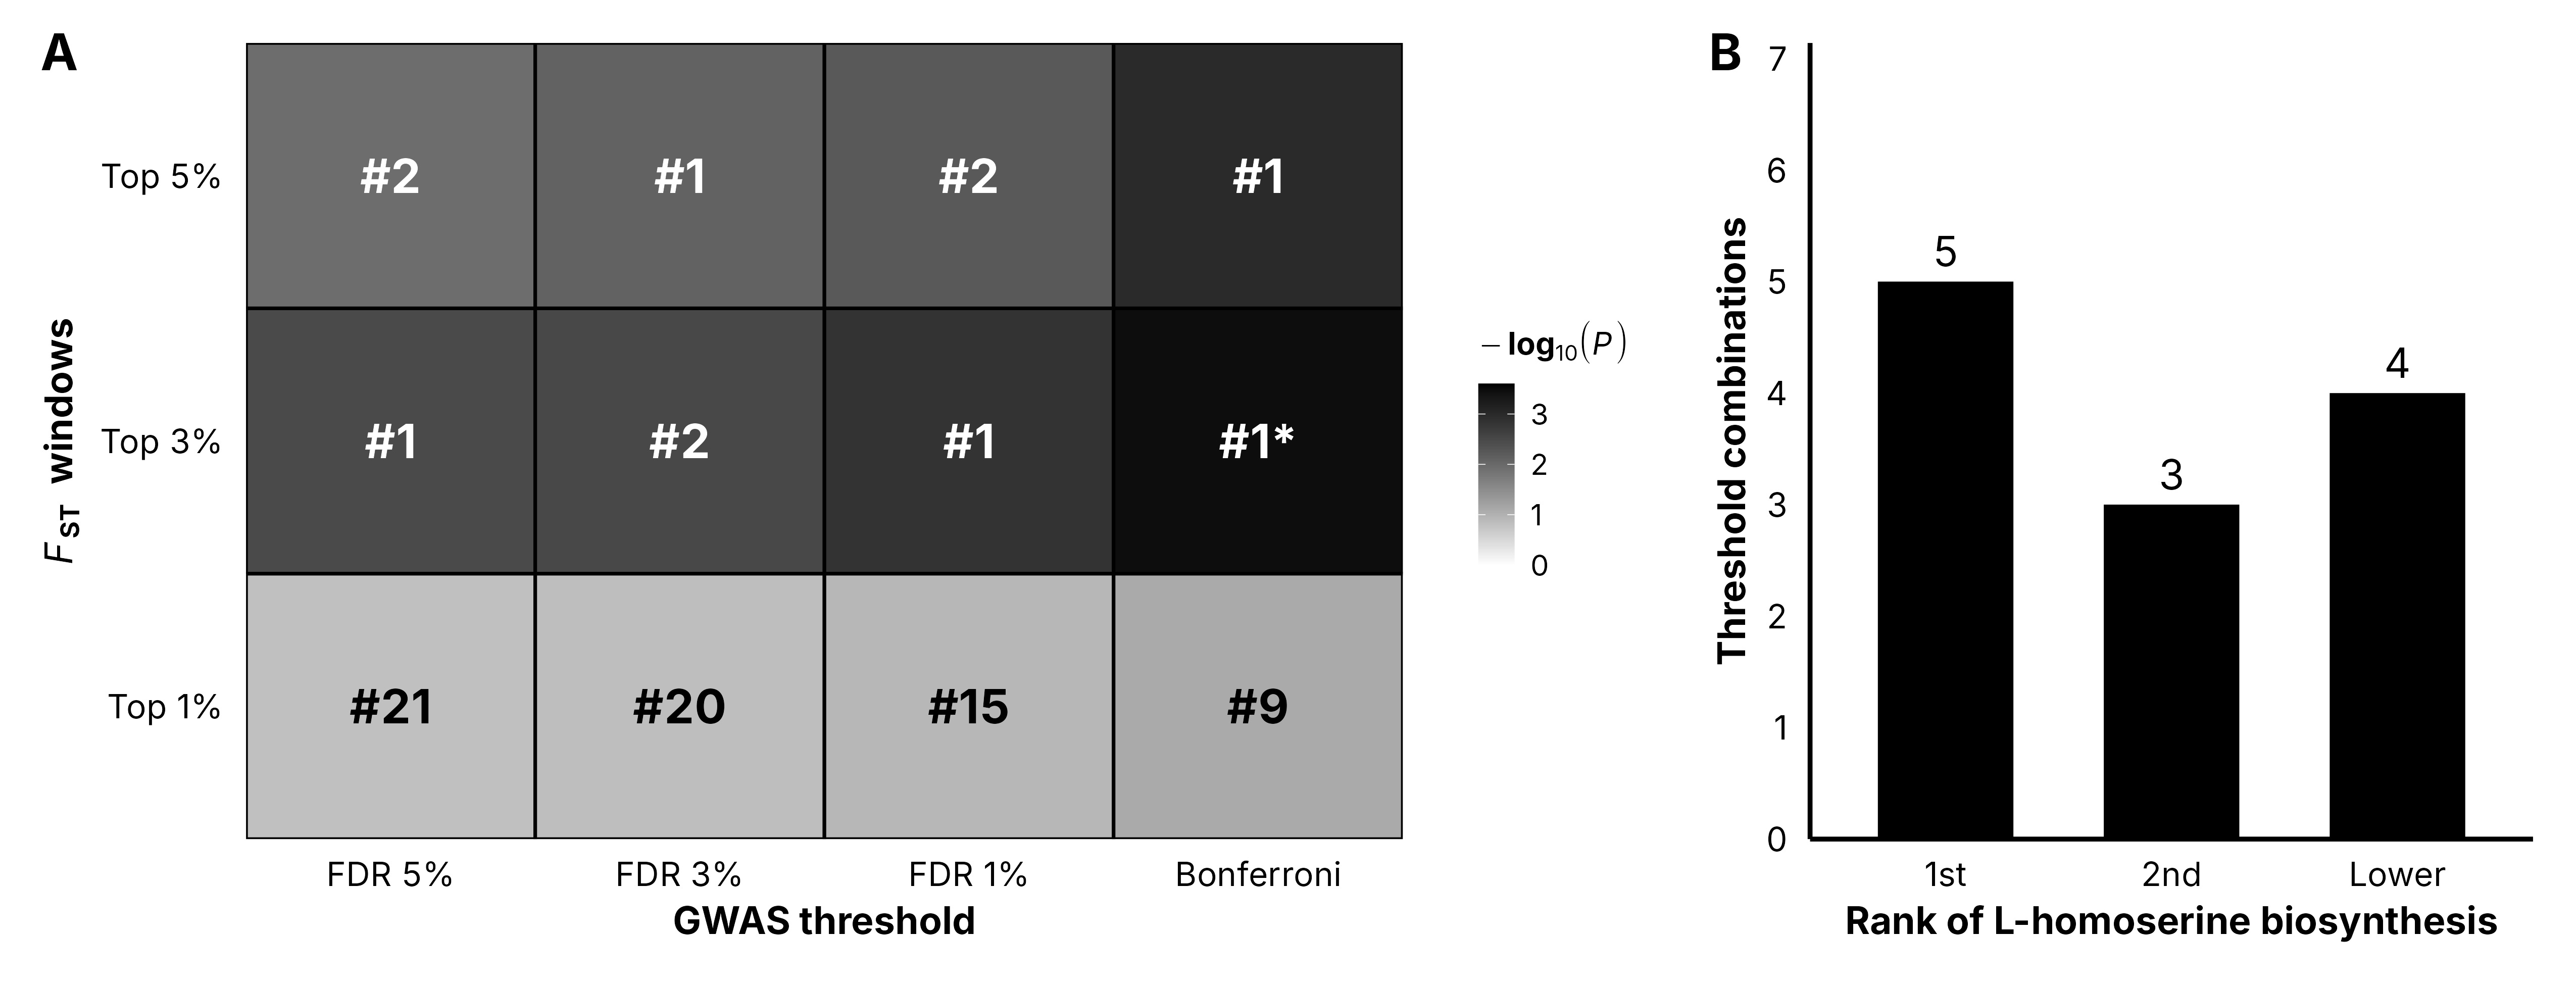
\includegraphics[width=0.75\textwidth]{../supp_figs/SuppFig_pathway_threshold_sensitivity.png}
\caption*{\textbf{Supplemental Figure S14.} \textbf{Sensitivity of the pathway recurrence test to candidate thresholds.} \textbf{(A)} L-homoserine biosynthesis across 12 combinations of GWAS threshold (columns, applied to both the amino acid and soil-N GWAS) and $F_{ST}$ window threshold (rows, Indian Chief and Jarvis). Shading gives $-\log_{10}$ of the pathway-specific permutation-based empirical $P$, labels give the rank of L-homoserine biosynthesis among the 468 CornCyc pathways, and an * marks $P < 0.05$ after correction across all pathways. At the top 1\%, the Indian Chief and Jarvis genes were no longer included and the pathway was hit by two analyses. \textbf{(B)} Number of the 12 combinations in which L-homoserine biosynthesis ranked first, second, or lower. Permutations, 20,000 per combination and 200,000 for the Bonferroni sets with the top 5\% and 3\% of windows.}
\end{figure}
\clearpage

\section*{Supplemental Tables}
Supplemental Tables S1--S22 are provided as separate CSV files.

\noindent\textbf{Supplemental Table S1.} \textbf{Free amino acid phenotypes across the Goodman--Buckler Association Panel.} Genotype-level values of the 78 amino acid phenotypes used for GWAS for 280 of the 282 lines (two years $\times$ two blocks, Columbia, Missouri): 20 absolute FAA concentrations, six biosynthetic-family composites, 20 ratios to the total free pool, 25 ratios to the family composite, four ratios between amino acids (N.D, N.E, N.Q, Q.E) and three whole-pool traits. Trait codes are defined in Supplemental Table~S2.

\noindent\textbf{Supplemental Table S2.} \textbf{Amino acid trait definitions.} Code and description of each of the 78 amino acid phenotypes in Supplemental Table~S1.

\noindent\textbf{Supplemental Table S3.} \textbf{Abundance, variability, and heritability of the 20 free amino acids.} For each FAA across 280 lines (278 for Tyr): median, mean, standard deviation, minimum, maximum, fold range, coefficient of variation, line mean broad-sense heritability ($H^2$), genomic heritability ($h^2$), and the Spearman correlation between 2017 and 2018 line means for the lines grown in both years.

\noindent\textbf{Supplemental Table S4.} \textbf{Heritability of free and protein-bound amino acid traits.} Line-mean and Cullis broad-sense heritability ($H^2$) and genomic heritability ($h^2$, with 95\% interval and permuted-phenotype null) for 40 FAA and 76 PBAA traits, with sample sizes and the Spearman correlation between 2017 and 2018 line means.

\noindent\textbf{Supplemental Table S5.} \textbf{Free vs.\ protein-bound amino acid pools.} Paired comparison of FAA and PBAA pools across matched lines for the total amino acid pool, the amino acid-derived N proxy, the proline fraction and the Asx + Glx + basic fraction (matched denominators): mean, median, standard deviation and coefficient of variation of each pool, fold difference and paired Wilcoxon $P$.

\noindent\textbf{Supplemental Table S6.} \textbf{Amino acid GWAS candidate genes.} All phenotype $\times$ SNP $\times$ gene combinations for SNPs significant at 5\% Benjamini--Hochberg FDR (per phenotype and model; MLM, BLINK, FarmCPU) within 25~kb of a B73 reference genome version 5 gene: 1,811 SNPs, 71 phenotypes, 3,693 genes. Includes significant models, lowest $P$ and FDR, whether the SNP is significant in $\geq$2 models, gene coordinates and distance. Positions are given on AGPv4 (\texttt{Pos\_v4}, the coordinate of the genotype data) and B73 reference genome version 5 (\texttt{Pos\_v5}, lifted with the chain file; \texttt{lift} = \texttt{gap} marks SNPs placed at the nearest aligned base); marker names carry the older AGPv3 coordinate.

\noindent\textbf{Supplemental Table S7.} \textbf{Amino acid GWAS loci.} The 2,152 loci were formed by merging FDR-significant SNP within 25 kb across phenotypes, with B73 reference genome version 5 coordinates, numbers of SNPs and phenotypes, best $P$, lead SNP (AGPv4 and v5 positions), supporting models, genes within 25 kb (or the nearest gene and its distance when none), top gene and its PANTHER family and GO terms.

\noindent\textbf{Supplemental Table S8.} \textbf{Genes in the chromosome~3 Asp/Pro QTL interval of the B64 $\times$ CML14 population.} The 1,578 B73 reference genome version 5 genes (1,386 protein-coding and 192 non-coding) within the 1.5-LOD support intervals (chr3:14.37--143.31~Mb) of the shared free Asp and Pro QTL (peak at 35.99~Mb), with gene coordinates, biotype, membership in the Asp and Pro intervals, distance to the QTL peak, gene name, PANTHER family, protein class, GO terms, kernel expression from qTeller \citep{qteller}, and overlap with candidates from the amino acid GWAS, soil N GWAS, and Indian Chief and Jarvis $F_{ST}$ scans.

\noindent\textbf{Supplemental Table S9.} \textbf{Soil N GWAS candidate genes.} The 448 B73 reference genome version 5 genes within 25~kb of the 216 soil-N SNPs (0--5~cm, 5\% FDR) that lie near a gene, one row per gene $\times$ SNP, with SNP statistics, overlap with other environmental GWAS, gene coordinates, distance, name, PANTHER family, protein class and GO terms.

\noindent\textbf{Supplemental Table S10.} \textbf{Environmental GWAS overlap test.} Observed vs.\ expected numbers of shared FDR-significant SNPs (MLM, BLINK and FarmCPU combined) for each site variable against the union of geographic variables (latitude, longitude, elevation; the variable itself excluded), and for soil N (0--5~cm) against each other variable. Expected $= n_1 n_2 / M$ with $M = 495{,}755$; one-sided hypergeometric $P$.

\noindent\textbf{Supplemental Table S11.} \textbf{Soil-N GWAS SNPs and their overlap with other environmental GWAS.} All 234 SNPs significant for soil N (0--5~cm) at 5\% FDR in MLM, BLINK or FarmCPU, with $P$ per model, MAF, number of models, whether each SNP is also FDR-significant in the GWAS of CEC, aridity, elevation, latitude, longitude, soil pH and soil N at 5--15~cm, and genes within 25~kb with the nearest gene's annotation.

\noindent\textbf{Supplemental Table S12.} \textbf{Genotype--environment correlation test for soil-N SNPs.} For each of the 234 soil-N SNPs, the Pearson correlation between genotype and soil N (0--5 and 5--15~cm), latitude, longitude, elevation, soil pH, CEC and aridity across 3,107 accessions; the SNP's genome-wide rank for each variable (\% of 495,755 SNPs with a stronger correlation); the most strongly correlated non-N variable; and the call: linked to environment (top 1\% for any non-N variable), not linked, or inconclusive (weak soil-N correlation, outside the top 5\%).

\noindent\textbf{Supplemental Table S13.} \textbf{Expectation test for the genotype–environment correlation.} Share of SNPs in the top 1\% of the genome for at least one geographic variable (latitude, longitude, elevation) or at least one of six non-N variables (adding soil pH, CEC, and aridity), for the whole genome, for SNPs in the top 1\% for correlation with soil N, for all soil N GWAS SNPs, and for those significant in $\geq$2 models, with binomial tests against the whole genome and against the soil N-correlated SNPs.

\noindent\textbf{Supplemental Table S14.} \textbf{Free amino acid metrics in Indian Chief and Jarvis, Cycle~0 vs. Cycle~14.} Eight pre-specified FAA metrics (total FAA per mg sample; Pro, Asn, Asp, Gln, and Gly fractions of total FAA; Asn + Gln + Arg + Lys + His per mg; FAA-derived N per mg) per population: biological-sample sizes, means, and medians per cycle, two-sided Wilcoxon rank-sum $P$, Benjamini--Hochberg-adjusted $P$ across the eight metrics, Cliff's $\delta$ (C14 vs. C0) and direction of change.

\noindent\textbf{Supplemental Table S15.} \textbf{Amino acid composition in Indian Chief and Jarvis, Cycle~0 vs.\ Cycle~14.} For each of the 20 free and 16 protein-bound amino acids, its fraction of the total pool per population and cycle: sample sizes, means, medians, Wilcoxon rank-sum $P$, Benjamini--Hochberg-adjusted $P$ across the amino acids of that pool, Cliff's $\delta$ and direction of change.

\noindent\textbf{Supplemental Table S16.} \textbf{Protein-bound amino acid metrics in Indian Chief and Jarvis, Cycle~0 vs.\ Cycle~14.} Six PBAA metrics (total PBAA per mg sample; proline, Asx and Glx fractions; Asx + Glx + Arg + Lys + His per mg; estimated PBAA-derived N per mg, with Asx and Glx at 1.5 N), with the same statistics as Supplemental Table~S14 and Benjamini--Hochberg adjustment across the six.

\noindent\textbf{Supplemental Table S17.} \textbf{Amino acid-derived N per mg sample in Indian Chief and Jarvis.} FAA-derived N, estimated PBAA-derived N, and estimated total amino acid-derived N per mg sample, per population and cycle, with Wilcoxon rank-sum $P$ and Benjamini--Hochberg-adjusted $P$ across the three measures.

\noindent\textbf{Supplemental Table S18.} \textbf{Indian Chief $F_{ST}$ windows, Cycle~0 vs. Cycle~14.} All 2,162 GenWin spline windows with chromosome, window number, start and end (B73 reference genome version 5), number of sites, mean per-site $F_{ST}$, whether the window is in the top 5\% ($F_{ST} \geq 0.157$), and the number and IDs of overlapping genes.

\noindent\textbf{Supplemental Table S19.} \textbf{Jarvis $F_{ST}$ windows, Cycle~0 vs.\ Cycle~14.} All 2,151 GenWin spline windows, with the same columns as Supplemental Table~S18 (top 5\%: $F_{ST} \geq 0.178$).

\noindent\textbf{Supplemental Table S20.} \textbf{Indian Chief candidate genes in top-5\% $F_{ST}$ windows.} The 2,001 genes overlapping the 109 top-5\% windows, with gene name, window coordinates and $F_{ST}$, whether the gene also lies in a top-5\% Jarvis window (\texttt{shared\_with\_other\_population}), PANTHER family and protein class, and Gene Ontology molecular function, biological process, and cellular component terms. Genes in the same window share one $F_{ST}$ value and are not independent.

\noindent\textbf{Supplemental Table S21.} \textbf{Jarvis candidate genes in top-5\% $F_{ST}$ windows.} The 1,179 genes overlap 106 of the 108 top-5\% windows (the other two contain no genes), with the same columns as Supplemental Table~S20.

\noindent\textbf{Supplemental Table S22.} \textbf{Expression responses of candidate genes to N supply in public maize RNA-seq.} Reanalysis of published maize RNA-seq studies of root, leaf, shoot, and whole-seedling tissue (no kernel data) for the candidate genes named in the text and \textit{ASN3}.


\bibliographystyle{oup-abbrvnat}
\bibliography{../../sn-bibliography}
\end{document}
